\documentclass[11pt]{article}
\usepackage[review]{acl}
\usepackage{times}
\usepackage{latexsym}
\usepackage[T1]{fontenc}
\usepackage[utf8]{inputenc}
\usepackage{microtype}
\usepackage{inconsolata}
\usepackage{graphicx}
\usepackage{amsmath}
\usepackage{amssymb}
\usepackage{booktabs}
\usepackage{multirow}
\usepackage{xcolor}
\usepackage{subcaption}
\usepackage{placeins}
\usepackage{float}
\usepackage{alphalph}
\usepackage{etoolbox}
\AtBeginEnvironment{figure}{\nolinenumbers}
\AfterEndEnvironment{figure}{\linenumbers}
\AtBeginEnvironment{figure*}{\nolinenumbers}
\AfterEndEnvironment{figure*}{\linenumbers}
\AtBeginEnvironment{table}{\nolinenumbers}
\AfterEndEnvironment{table}{\linenumbers}
\AtBeginEnvironment{table*}{\nolinenumbers}
\AfterEndEnvironment{table*}{\linenumbers}

\graphicspath{{../figures/paper/}{../artifacts/}}

\title{Exposure Bias Collapses Auxiliary Attention Losses in Multi-Turn Dialogue}

\author{Anonymous}

\begin{document}
\maketitle

\begin{abstract}
As multi-turn conversations grow longer, large language models progressively lose attention to the system-prompt goals that define their task, even when the underlying goal representations remain intact. Existing remedies operate at inference time, leaving a natural but untested alternative: training auxiliary attention losses alongside next-token prediction to directly optimize goal attention. This strategy assumes that attention patterns learned under teacher forcing will transfer to autoregressive generation, an assumption that classical exposure bias research has challenged for sequence models but that has never been examined for auxiliary attention objectives in multi-turn transformers.
We show this assumption fails. On a controlled five-way testbed spanning two architectures (Qwen-2.5-7B, Llama-3.1-8B), goal attention optimized to target under teacher forcing collapses by an order of magnitude under autoregressive generation. A diagnostic exclusion chain traces the failure to exposure bias, ruling out gradient conflict, gating mechanism, and parameter capacity as primary causes. Inference-time attention steering confirms that the collapse reflects attention misallocation rather than representation loss. Scheduled sampling, applied here for the first time to auxiliary attention objectives in multi-turn transformers, compresses the training--inference gap to near parity on Qwen and from ${\sim}$27$\times$ to 2.9$\times$ on Llama, with no perplexity cost\footnote{Code and data are available at \url{https://anonymous.4open.science/r/turn_residual_gating-8703/}.}.
\end{abstract}

\section{Introduction}\label{sec:introduction}

Multi-turn dialogue is central to how large language models are deployed, from customer service to tutoring to long-form reasoning. Yet a persistent failure accompanies even the most fluent generation: as conversations grow longer, models pay progressively less attention to the system-prompt goals that define their task. \citet{dongre2026attention} measured significant Goal Accessibility Ratio (GAR) decline across 12 models over extended conversations; in our own evaluation, goal attention drops by over 70\% within just five turns. Crucially, this is not a representation problem: residual stream probes confirm that goal information persists (AUC\,=\,0.98). The model retains the knowledge of what it should attend to; it simply stops attending.

Existing remedies address this decay at inference time. Split-softmax \citep{li2024measuring} separates instruction from conversation tokens; StreamingLLM \citep{xiao2024streaming} retains anchor tokens; Gated Attention \citep{qiu2025gated} applies per-head sigmoid gates within a single forward pass. A natural alternative is to intervene during training: optimize goal attention directly through auxiliary losses trained alongside next-token prediction (NTP). Yet this strategy rests on an untested assumption: attention patterns learned under teacher forcing (TF) transfer to autoregressive (AR) generation. Classical exposure bias research \citep{bengio2015scheduled,lamb2016professor} has shown that TF creates a training--inference distribution mismatch for RNN sequence models, but whether this mismatch extends to auxiliary attention objectives in multi-turn transformers remains unknown.

We test this assumption and find it fails. We introduce a controlled five-way testbed (ThreadGate, +PCGrad \citep{yu2020pcgrad}, Uniform Gate, LoRA-only, and Base) designed not as competing solutions but as a diagnostic exclusion chain (\S\ref{sec:comparison-design}), where each adjacent pair isolates one candidate failure mechanism. The result is unambiguous: every variant converges to target GAR under teacher forcing, yet goal attention collapses by an order of magnitude once the model generates its own context (Figure~\ref{fig:headline}). The exclusion chain traces this collapse to exposure bias, the training--inference distribution mismatch, ruling out gradient direction conflict (PCGrad removes conflict yet \emph{worsens} AR GAR), gating mechanism (Uniform Gate matches ThreadGate), and parameter capacity (LoRA-only shows the same pattern). Inference-time $\beta$-steering confirms that the collapse reflects attention misallocation rather than representation degradation; scheduled sampling bridges the gap by exposing the model to its own generations during training.

\begin{figure*}[!ht]
  \centering
  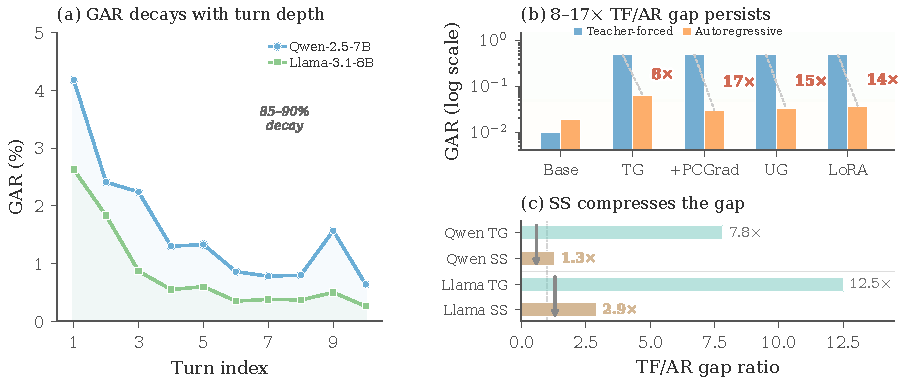
\includegraphics[width=\textwidth]{fig1_headline.pdf}
  \caption{Exposure bias collapses auxiliary attention losses. \textbf{(a)}~Goal attention decays 85--90\% across turns under AR generation on both Qwen-2.5-7B and Llama-3.1-8B. \textbf{(b)}~Under TF evaluation all variants reach GAR$\approx$0.50, but AR generation collapses GAR by 8--17$\times$ (log scale). \textbf{(c)}~Scheduled sampling compresses the TF--AR gap from 7.9$\times$ to 1.3$\times$ (Qwen, 3-seed mean) and ${\sim}$27$\times$ to 2.9$\times$ (Llama).}
  \label{fig:headline}
\end{figure*}

Our contributions are:
\begin{enumerate}\raggedright
    \item \textbf{Exposure bias characterization.} To our knowledge, the first empirical demonstration that exposure bias collapses auxiliary attention objectives in multi-turn transformers, with an order-of-magnitude TF--AR gap reproduced across two architectures (Qwen-2.5-7B, Llama-3.1-8B) and model scales (1.5B--8B).
    \item \textbf{Diagnostic exclusion testbed.} A five-way diagnostic design, informed by seven loss-formulation iterations, that isolates the failure mechanism via systematic diagnostic exclusion, including a PCGrad \emph{modus tollens} argument ruling out gradient direction conflict ($p$\,=\,0.002, effect reverses).
    \item \textbf{Attention misallocation diagnosis.} Inference-time $\beta$-steering recovers goal attention with modest perplexity cost, evidence that the collapse is an attention routing failure, not a representational one.
    \item \textbf{Scheduled sampling as remedy.} The first application of scheduled sampling to auxiliary attention objectives in multi-turn transformers, compressing the TF--AR gap to ${\sim}$1.3$\times$ on Qwen (3-seed mean) and ${\sim}$2.9$\times$ on Llama with no perplexity degradation, robust across three seeds.
\end{enumerate}

\section{Related Work}\label{sec:related}

\paragraph{Multi-turn dialogue and attention decay.}
Multi-turn coherence has been a persistent challenge from early dialogue systems \citep{li2016persona,roller2021recipes,zhang2020dialogpt} through modern long-context models \citep{xu2022goldfish}, with benchmarks such as MT-Bench \citep{zheng2024judging} and MT-Bench-101 \citep{bai2024mtbench101} continuing to expose quality gaps at later turns \citep{laban2025lost,liu2026intent}. Most relevant to our work, \citet{dongre2026attention} defined the Goal Accessibility Ratio (GAR) and showed that attention to goal tokens decays 27--48\% across 12 models while residual probes retain goal information (AUC\,=\,0.98). We observe a steeper 70.8\% decline on Qwen-2.5-7B. \citet{li2024measuring} independently quantified instruction instability and proposed split-softmax as an inference-time remedy. Our work differs in scope: we diagnose \emph{why} training-time attention optimization fails to transfer to inference, and provide the first training-time mitigation.

\paragraph{Gating and attention manipulation.}
Residual gating spans highway networks \citep{srivastava2015highway}, ReZero \citep{bachlechner2021rezero}, layer pruning \citep{gromov2024unreasonable,fan2020layerdrop}, and adaptive depth \citep{schuster2022calm,raposo2024mixture}. Most relevant is Gated Attention \citep{qiu2025gated}: per-head sigmoid gates achieving MMLU \citep{hendrycks2021measuring} $+$2.03 at 15B scale; ThreadGate differs in conditioning on turn position. On the analysis side, head specialization \citep{clark2019what,voita2019analyzing,kovaleva2019revealing}, positional bias calibration \citep{liu2024lost,xiao2024streaming}, and attention steering (PASTA; \citealp{zhang2024tell}) address inference behavior; our $\beta$-steering serves a diagnostic role. PCGrad \citep{yu2020pcgrad} and CAGrad \citep{liu2021cagrad} treat gradient conflict as the root cause; we show direction conflict is a symptom, not the primary cause.

\paragraph{Exposure bias in sequence models.}
Teacher forcing creates a distributional mismatch between training and inference \citep{wiseman2016sequence,arora2022exposure}. Scheduled sampling \citep{bengio2015scheduled} introduced curriculum-based mixing; subsequent work proposed sequence-level objectives \citep{ranzato2016sequence}, adversarial regularization \citep{lamb2016professor}, self-recovery analysis \citep{he2019exposure}, bridging strategies for neural machine translation (NMT; \citealp{zhang2019bridging}), and search-based training \citep{leblond2018searnn}. \citet{mihaylova2019scheduled} extended scheduled sampling to transformers for single-turn NMT. \citet{dou2019attention} proposed attention forcing (supervising cross-attention during NMT), and \citet{dou2022parallel} extended it with KL-divergence switching. Our work differs: (i)~time-scheduled sampling (linearly increasing mixing ratio), not data-dependent; (ii)~self-attention in multi-turn dialogue, not cross-attention in NMT; (iii)~auxiliary attention objectives, not primary translation loss. No prior work examines exposure bias on \emph{auxiliary} attention objectives or provides multi-turn transformer mitigation; we fill both gaps.

\begin{table*}[!t]
\centering
\small
\caption{Five-way comparison on Qwen-2.5-7B-Instruct. TF evaluation uses IID UltraChat and 50 held-out conversations; AR evaluation uses $N$\,=\,50 held-out conversations (mean 3.6 user turns). All fine-tuned variants converge under TF ($\leq$2\,pp spread); the 8--17$\times$ TF-AR gap persists across all configurations. $\bar{g}\!\pm\!\sigma_g$: learned gate mean and std across 28 layers (LoRA-only has no gates). GAR-O = GAR-ours; GAR-D = GAR-Dongre \citep{dongre2026attention}; PPL = perplexity.}
\label{tab:five-way}
\begin{tabular}{l ccc ccc cc c}
\toprule
& \multicolumn{3}{c}{\textbf{IID (TF)}} & \multicolumn{3}{c}{\textbf{Held-out (TF)}} & \multicolumn{2}{c}{\textbf{AR ($N$\,=\,50)}} & \\
\cmidrule(lr){2-4} \cmidrule(lr){5-7} \cmidrule(lr){8-9}
\textbf{Configuration} & GAR-O & GAR-D & PPL & GAR-O & GAR-D & PPL & GAR-O & 95\% CI & $\bar{g}\!\pm\!\sigma_g$ \\
\midrule
\multicolumn{10}{l}{\emph{Baseline}} \\
Base              & 0.01 & 0.00 & 4.23 & 0.01 & 0.00 & 4.34 & 0.019 & {\scriptsize[.014,\,.024]} & --- \\
\midrule
\multicolumn{10}{l}{\emph{Gated variants}} \\
ThreadGate        & 0.49 & \textbf{0.02} & 2.63 & 0.50 & \textbf{0.02} & 2.78 & \textbf{0.064} & {\scriptsize[.041,\,.091]} & .93\,{\scriptsize$\pm$\,.05} \\
\;+\,PCGrad       & 0.50 & 0.01 & 2.78 & 0.50 & 0.01 & 2.78 & 0.030 & {\scriptsize[.023,\,.038]} & --- \\
Uniform Gate      & 0.49 & 0.01 & 2.62 & \textbf{0.51} & 0.01 & 2.78 & 0.033 & {\scriptsize[.025,\,.043]} & .96\,{\scriptsize$\pm$\,.05} \\
\midrule
\multicolumn{10}{l}{\emph{Ungated}} \\
LoRA-only         & 0.49 & 0.01 & 2.63 & 0.50 & 0.01 & 2.78 & 0.037 & {\scriptsize[.027,\,.050]} & 1.00 \\
\bottomrule
\end{tabular}
\end{table*}

\section{Method}\label{sec:method}

\subsection{Preliminaries}\label{sec:background}

\paragraph{Goal Accessibility Ratio.}
Standard metrics such as perplexity and attention entropy capture generation quality but not \emph{what} the model attends to. In multi-turn dialogue, a model may generate fluent text while progressively ignoring task specifications in the system prompt. We need a metric that directly measures whether goal-relevant context receives attention. To formalize this, we denote the task specification tokens in the system prompt as \emph{goal tokens} $\mathcal{G}$. \citet{dongre2026attention} defined the Goal Accessibility Ratio (GAR) for a model with $L$ layers and $H$ heads at turn $\tau$ as
\begin{equation}\label{eq:gar}
  \text{GAR}(\tau) = \frac{1}{L \cdot H \cdot |\mathcal{R}_\tau|} \sum_{\ell=1}^{L} \sum_{h=1}^{H} \sum_{i \in \mathcal{R}_\tau} \sum_{j \in \mathcal{G}} A_{i,j}^{(\ell,h)},
\end{equation}
where $\mathcal{R}_\tau$ is the set of response tokens at turn $\tau$ and $A_{i,j}^{(\ell,h)}$ is the attention weight from token $i$ to token $j$ at layer $\ell$, head $h$.

\paragraph{Two GAR variants.}
\textbf{GAR-Dongre} is the original definition (Eq.~\ref{eq:gar}), averaging over all response tokens. However, averaging dilutes the signal with intermediate positions that may legitimately attend to local context rather than the system prompt. The last token of each assistant turn is where the model aggregates information for the next continuation; attention at this position most directly reflects the model's awareness of task specifications. \textbf{GAR-ours} restricts the measurement accordingly:
\begin{equation}\label{eq:gar-ours}
  \text{GAR\text{-}ours}(\tau) = \frac{1}{L \cdot H} \sum_{\ell=1}^{L} \sum_{h=1}^{H} \sum_{j \in \mathcal{G}} A_{t_\tau,\, j}^{(\ell,h)},
\end{equation}
where $t_\tau$ is the last token index at turn $\tau$. Attention at this position reflects the information drawn upon for continuation; we use GAR-ours as the optimization target for $\mathcal{L}_\text{GAR}$ (\S\ref{sec:loss}). Empirically, GAR-Dongre is diluted by NTP attention patterns to ${\sim}$0.01--0.02 in multi-turn settings, losing discriminative power across configurations; GAR-ours retains an order-of-magnitude range (0.019--0.50). The contrast itself is informative: goal attention concentrates at the last-token position, and only this concentrated pattern is vulnerable to distribution shift (\S\ref{sec:analysis}). Throughout this work, GAR serves primarily as a \emph{diagnostic probe}: it measures whether auxiliary attention training transfers to autoregressive generation, rather than being an end-to-end optimization objective whose increase directly improves downstream task performance (the correlation with instruction retention is weak; $r$\,=\,0.200, $p$\,=\,0.007; \S\ref{sec:discussion}).

\subsection{ThreadGate Architecture}

\begin{figure}[t]
  \centering
  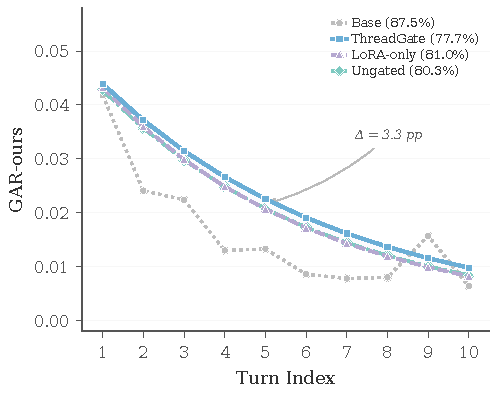
\includegraphics[width=\columnwidth]{fig4_attention_heatmap.pdf}
  \caption{Per-turn GAR-ours under AR generation ($N$\,=\,5 conversations, 10 turns). All fine-tuned variants cluster together (77--81\% decay; $\Delta$\,=\,3.3\,pp between ThreadGate and LoRA-only); Base decays 87.5\%. Gating adds zero incremental effect.}
  \label{fig:attention-heatmap}
\end{figure}

Different transformer layers serve different roles: early layers capture local syntax while later layers integrate long-range context \citep{gromov2024unreasonable}. A global intervention would uniformly scale all layers, but goal attention decay is layer-dependent: some layers contribute more to cross-turn information routing than others. ThreadGate therefore adds a \emph{per-layer} gating mechanism to the residual stream, allowing the model to learn which layers to modulate. At each layer $l$, the residual update is scaled by a scalar gate:
\begin{equation}
  x_{l+1} = x_l + g_l \cdot f_l(x_l),
\end{equation}
where $f_l$ denotes the sublayer computation (self-attention or feed-forward network, FFN). Since residual networks can be viewed as ensembles of shallow paths \citep{veit2016residual}, per-layer gating selectively modulates individual paths within this ensemble. This resembles ReZero \citep{bachlechner2021rezero}, which initializes a single trainable scalar at zero to stabilize deep network training, but ThreadGate differs in three ways: (i)~gates are \emph{content-conditioned}, a function of the hidden state rather than a fixed scalar; (ii)~gates are \emph{turn-conditioned}, incorporating conversation-position features; (iii)~gates are initialized near identity ($\sigma(1.5) \approx 0.82$) rather than zero, preserving the pretrained model's computation.

Concretely, each gate $g_l$ is produced by a two-layer MLP that takes both content and turn features as input:
\begin{align}\label{eq:gate}
  g_l = \sigma\bigl(W_2\,\text{ReLU}(&W_1\,[\text{proj}(x_l);\;\text{emb}(t_d, t_i)] \notag\\
  &+ b_1) + b_2\bigr),
\end{align}
where $\text{proj}(\cdot)$ reduces the hidden dimension to 16, and $\text{emb}(t_d, t_i)$ provides a 16-dimensional turn embedding encoding turn distance $t_d$ (turns since system prompt) and turn index $t_i$ via learned lookup tables. The 32-dimensional input passes through a 64-unit hidden layer to a scalar gate in $(0, 1)$ via sigmoid. For Qwen-2.5-7B ($L\!=\!28$), this adds ${\sim}$57K parameters ($<$0.001\% of 7B). To isolate the contribution of turn conditioning, the \textbf{Uniform Gate} ablation replaces $\text{emb}(\cdot)$ with a learnable constant, removing turn awareness while retaining content-conditioned gating. To preserve pretrained behavior, gate biases are initialized to 1.5 (${\sim}$82\% pass-through) rather than zero as in ReZero, and gate parameters receive a $10\times$ learning rate multiplier to accelerate adaptation.

\subsection{Training Objective}\label{sec:loss}

Next-token prediction alone provides no gradient signal for attention allocation; a model can achieve low perplexity while distributing attention arbitrarily. The auxiliary GAR loss provides explicit pressure to maintain goal-token attention, while a diversity regularizer prevents gate collapse. The training objective combines three terms:
\begin{equation}
  \mathcal{L} = \mathcal{L}_\text{NTP} + \lambda_\text{GAR}\,\mathcal{L}_\text{GAR} + \lambda_\text{div}\,\mathcal{L}_\text{div}.
\end{equation}
$\mathcal{L}_\text{NTP}$ is the standard next-token prediction loss. For $\mathcal{L}_\text{GAR}$, we use MSE rather than cross-entropy because GAR is a continuous ratio and MSE provides \emph{bidirectional} pressure, penalizing both under- and over-attention and preventing identity collapse (Appendix~\ref{sec:appendix-loss}):
\begin{equation}
  \mathcal{L}_\text{GAR} = \text{MSE}(\text{GAR\text{-}ours}, \tau),
\end{equation}
where $\tau = 0.5$ targets allocating half of the last token's attention to goal tokens. Without diversity pressure, all gates converge near 1.0; the gate diversity loss prevents this:
\begin{equation}
  \mathcal{L}_\text{div} = \text{ReLU}(\sigma_\text{min} - \text{std}(\mathbf{g})),
\end{equation}
where $\mathbf{g} = [g_1, \ldots, g_L]$ and $\sigma_\text{min} = 0.05$ is a minimum standard deviation threshold ($\lambda_\text{GAR} = \lambda_\text{div} = 1.0$). This formulation emerged from seven iterations spanning four loss families (Appendix~\ref{sec:appendix-loss}): cumulative (v1--v2) and maximize (v3--v6) objectives either starve gate gradients at equilibrium or drive gates toward identity; only MSE provides the bidirectional pressure needed to prevent identity collapse.

\subsection{Controlled Comparison Design}\label{sec:comparison-design}

We design a five-way comparison where each adjacent pair isolates one factor: \textbf{ThreadGate (TG) vs.\ Uniform Gate (UG)} (turn conditioning), \textbf{TG vs.\ LoRA-only} (gating mechanism), \textbf{ThreadGate vs.\ +PCGrad} (gradient conflict via gradient surgery \citep{yu2020pcgrad}), and \textbf{Fine-tuned vs.\ Base} (LoRA adaptation). All fine-tuned variants share training data, LoRA configuration, optimizer, and seed (Appendix~\ref{sec:appendix-hyper}).


\section{Experiments}
\label{sec:experiments}

\subsection{Setup}

We fine-tune Qwen-2.5-7B-Instruct with LoRA \citep{hu2022lora,dettmers2023qlora} on 8K multi-turn conversations from the UltraChat \citep{ding2023ultrachat} training split. Training uses 3 epochs with AdamW (lr $= 2 \times 10^{-4}$, batch size 1, gradient accumulation 8, seed 42; ThreadGate additionally with seed 123); each variant requires approximately 6 hours on a single NVIDIA RTX PRO 6000 Blackwell Server Edition GPU (96\,GB; training costs in Appendix~\ref{sec:appendix-cost}). Full hyperparameters are in Appendix~\ref{sec:appendix-hyper}; dataset statistics in Appendices~\ref{sec:appendix-data} and~\ref{sec:appendix-dataset-ext}; the controlled comparison design is described in \S\ref{sec:comparison-design}. We evaluate under \emph{IID} (same-distribution UltraChat text) and \emph{held-out} (50 non-overlapping conversations) teacher-forced protocols, reporting GAR-ours, GAR-Dongre \citep{dongre2026attention}, and perplexity (PPL).

\subsection{Main Results}

Table~\ref{tab:five-way} presents the five-way comparison. Under TF evaluation, all fine-tuned variants converge: GAR-ours spans 0.49--0.51 ($\leq$2\,pp), PPL is 2.62--2.78. IID and held-out protocols produce identical rankings (held-out GAR-ours differs by $\leq$2\,pp), ruling out data overlap as a confound. GAR-Dongre remains low (0.01--0.02) with no TF-AR gap, indicating that only concentrated last-token attention is vulnerable to distribution shift; scheduled sampling breaks this pattern (\S\ref{subsec:ss}).

Under AR generation ($N$\,=\,50), GAR-ours drops to 0.019--0.064, an 8--17$\times$ gap (Figure~\ref{fig:headline}). The ordering (ThreadGate 0.064 $>$ LoRA-only 0.037 $>$ Uniform Gate 0.033 $>$ PCGrad 0.030 $>$ Base 0.019) shows ThreadGate vs.\ LoRA-only is significant ($p$\,=\,0.004; Appendices~\ref{sec:appendix-stats} and~\ref{sec:appendix-stats-ext}), yet the gap remains 7.9$\times$. A second seed confirms TF stability ($0.504\pm0.001$). MMLU 5-shot accuracy remains within 0.8\,pp across all variants (per-category breakdown in Appendix~\ref{sec:appendix-mmlu-ext}). We analyze this distribution shift in \S\ref{sec:analysis}.

\begin{figure*}[!t]
  \centering
  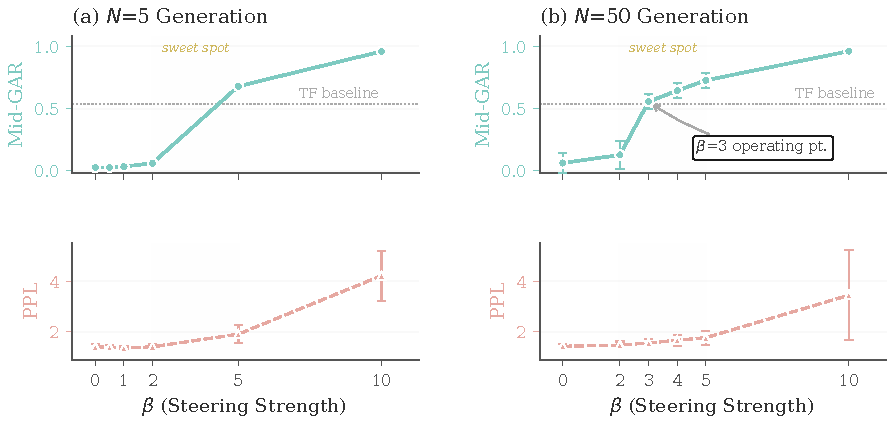
\includegraphics[width=\textwidth]{fig5_attention_steering.pdf}
  \caption{Inference-time $\beta$-steering recovers GAR from 0.064 to 0.727, consistent with attention misallocation as a proximal cause (9\% PPL cost at $\beta$\,=\,3; phase transition at $\beta \in [2, 3]$).}
  \label{fig:steering-recovery}
\end{figure*}

\subsection{Inference-Time Attention Steering}\label{subsec:steering}

All training-time interventions leave the exposure bias gap intact. If the collapse is caused by attention misallocation rather than representation degradation, then directly correcting attention should recover GAR. We test this by adding a constant bias $\beta$ to pre-softmax attention logits for goal-token positions during generation:
\begin{equation}
  \tilde{A}_{i,j}^{(\ell,h)} = A_{i,j}^{(\ell,h)} + \beta \cdot \mathbf{1}[j \in \mathcal{G}],
\end{equation}
where $\tilde{A}$ denotes the modified logits before softmax. The additive form operates in log-probability space, providing uniform boost even when baseline attention is near zero. The response is sharply nonlinear: $\beta \in [0, 2]$ yields marginal improvement, then $\beta = 3$ triggers a phase transition to GAR\,=\,0.556 (9\% PPL cost). At $\beta$\,=\,5, GAR reaches 0.727$\pm$0.061 (PPL 1.77); the operating region $\beta \in [3, 5]$ exceeds the TF baseline while PPL remains below 1.8 (Figure~\ref{fig:steering-recovery}; full results in Appendix~\ref{sec:appendix-steering}; per-$\beta$ turn-level trajectories in Appendix~\ref{sec:appendix-steering-viz}). GAR recovery under steering is partly by construction: boosting attention logits toward goal tokens mechanically increases the attention-based metric. The stronger evidence is the counterfactual: if the collapse were due to hidden-state drift rather than attention misallocation, reweighting could not recover GAR, yet it does, consistent with attention misallocation as a proximal cause (qualitative examples in Appendix~\ref{sec:appendix-examples}). Downstream, steering ($\beta$\,=\,3) raises late-turn instruction compliance by +11.1\,pp, though this effect does not reach conventional significance ($p$\,=\,0.077; content-constrained tasks benefit most, +23.8\,pp; Appendix~\ref{sec:appendix-ir}).

\subsection{Scheduled Sampling Compresses the TF--AR Gap}\label{subsec:ss}

\begin{figure}[t]
  \centering
  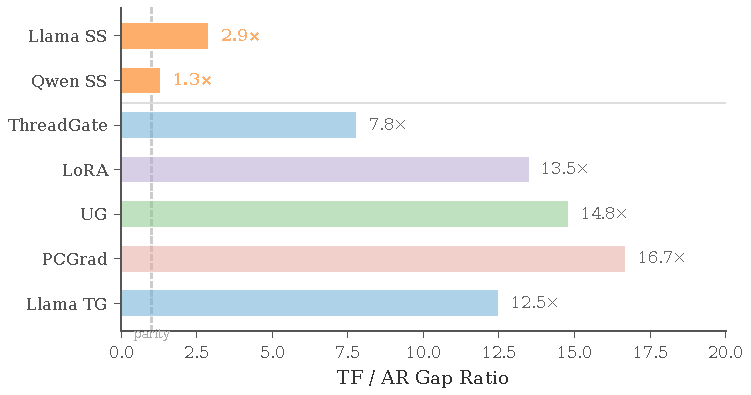
\includegraphics[width=\columnwidth]{fig_ss_gap_compression.pdf}
  \caption{Scheduled sampling compresses the TF-AR gap from 7.9$\times$ to ${\sim}$1.3$\times$ (3-seed mean), the only variant approaching parity across five training conditions.}
  \label{fig:ss-gap}
\end{figure}

Scheduled sampling (SS; \citealp{bengio2015scheduled}), which mixes model-generated tokens into training prefixes with linearly increasing probability (Appendix~\ref{sec:appendix-ss}), directly targets the training-inference mismatch. Across three seeds, AR GAR-ours rises to $0.401\pm0.047$, compressing the gap from 7.9$\times$ to ${\sim}$1.3$\times$ (TF GAR $0.517\pm0.032$; 3-seed mean) with no PPL cost ($1.441\pm0.002$; Figure~\ref{fig:ss-gap}; per-seed details in Appendix~\ref{sec:appendix-perseed}). Steering on SS models nearly eliminates seed variance ($\beta$\,=\,5: $0.717\pm0.001$, std 0.047$\to$0.001; Figure~\ref{fig:ss-multiseed}). SS generalizes across GAR definitions (mid-turn GAR above 0.36 for all token-position variants; Appendix~\ref{sec:appendix-gar-robust}; extended robustness in Appendix~\ref{sec:appendix-gar-ext}) and across architectures: on Llama-3.1-8B, SS compresses the gap from ${\sim}$27$\times$ to 2.9$\times$, weaker than Qwen likely due to fewer training epochs (2 vs.\ 3; \S\ref{subsec:cross-model}). The benefit diminishes in longer dialogues (Appendix~\ref{sec:appendix-n5}), consistent with exposure bias compounding over turns.



\section{Analysis}\label{sec:analysis}

\begin{figure*}[!t]
  \centering
  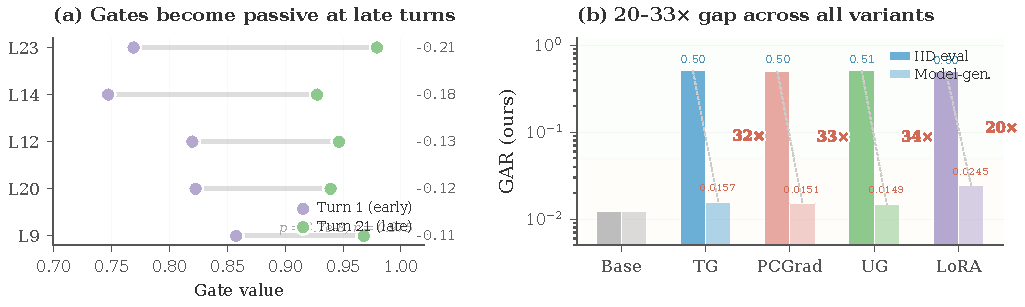
\includegraphics[width=\textwidth]{fig3_gate_shift.pdf}
  \caption{(a)~Gate turn conditioning: per-layer gate values at turn~1 vs turn~21. In 27/28 layers, gates approach 1.0 at late turns, inverting the design intent ($p = 3.73 \times 10^{-8}$). (b)~Distribution shift ($N$\,=\,5 pilot): the TF-AR GAR gap persists across all five variants. Pilot gaps (20--34$\times$) exceed final $N$\,=\,50 estimates (8--17$\times$; Table~\ref{tab:five-way}) due to smaller sample size.}
  \label{fig:gate-shift}
\end{figure*}

Each subsection kills one alternative hypothesis via diagnostic exclusion: \S\ref{subsec:gate-conditioning}~turn conditioning, \S\ref{subsec:pcgrad}~gradient direction conflict, leaving exposure bias as the primary remaining explanation consistent with current evidence (\S\ref{subsec:dist-shift}). \S\ref{subsec:mechanism-specificity} confirms selectivity; \S\ref{subsec:cross-model} confirms cross-architecture generalization.

\subsection{Gate Turn Conditioning}\label{subsec:gate-conditioning}

We compare gate values at turn~1 (early) and turn~21 (late) across all 28 layers. The gates invert the design intent: in 27/28 layers, gate values are \emph{lower} at turn~1 than turn~21 (Wilcoxon $p = 3.73 \times 10^{-8}$, $r = 0.975$); e.g., layer~23 shifts from 0.769 to 0.979. NTP pressure pushes gates toward 1.0, a convergence pattern reminiscent of attention collapse in deep transformers \citep{dong2021attention}, yielding inference-time values of 0.93--0.98 (2--7\% attenuation; Table~\ref{tab:five-way}; full gate profiles in Appendix~\ref{sec:appendix-gate-profile}; training dynamics in Appendix~\ref{sec:appendix-training-ext}). The Uniform Gate learns comparable per-layer variation (L3\,=\,0.777, L27\,=\,1.000) despite lacking turn conditioning; the structure thus arises from LoRA$+$GAR pressure (Figure~\ref{fig:gate-shift}a). Does the NTP-GAR gradient conflict prevent the intended behavior?

\subsection{PCGrad Gradient Direction Conflict Exclusion}\label{subsec:pcgrad}

NTP and GAR gradients oppose in 68--79\% of layers (cosine similarity $-$0.089$\to$$-$0.042 across epochs), with NTP magnitude dominance growing from 7.5$\times$ to 14.7$\times$ (full gradient statistics in Appendix~\ref{sec:appendix-gradient}). If this direction conflict prevents GAR convergence, eliminating it via PCGrad \citep{yu2020pcgrad}, which projects conflicting gradients onto the other's normal plane, should prevent the collapse. To our knowledge, this is the first application of PCGrad as a \emph{diagnostic} tool rather than an optimization method.

PCGrad shifts cosine similarity to oscillate around zero, yet TF metrics are unchanged. AR GAR \emph{worsens}: 0.064$\to$0.030 ($p$\,=\,0.002; Figure~\ref{fig:training-pcgrad}b in Appendix~\ref{sec:appendix-gradient}). By \emph{modus tollens}: removing gradient direction conflict does not prevent collapse; therefore it is not the primary cause. PCGrad eliminates direction conflict but does not address magnitude imbalance (NTP dominates GAR by 7.5--14.7$\times$); the worsening under PCGrad may partly reflect projection side-effects rather than confirming that direction conflict is entirely absent as a factor. Cross-model analysis confirms this pattern: Llama-3.1-8B gradients are near-orthogonal (cos\,=\,+0.005) with 25.7$\times$ NTP magnitude dominance (Table~\ref{tab:gradient-crossmodel}).

\subsection{Distribution Shift Analysis}\label{subsec:dist-shift}

The TF-AR GAR gap persists across all variants (Table~\ref{tab:five-way}). GAR-Dongre provides a control: it remains uniformly low (0.01--0.02) with no distribution gap, evidence that the shift selectively destroys concentrated last-token attention. The mechanism is exposure bias \citep{bengio2015scheduled,zhang2019bridging,arora2022exposure}: during training the model conditions on ground-truth prefixes; at inference, on its own outputs. GAR optimizes a distributional property with no autoregressive counterpart, explaining why TF GAR-ours remains near $\tau$\,=\,0.5 while AR GAR collapses (77--87\% per-turn decay; Figure~\ref{fig:attention-heatmap}; per-configuration AR trajectories in Appendix~\ref{sec:appendix-ar-gar-dynamics}; scaling analysis in Appendix~\ref{sec:appendix-eb-scaling}).

\subsection{Mechanism Specificity}\label{subsec:mechanism-specificity}

We test specificity with Turn-level Residual Coherence (TRC), the cosine similarity between adjacent-turn hidden states. TF/AR TRC is 0.334/0.332 for ThreadGate (gap $+$0.002) and 0.349/0.411 for LoRA-only (gap $-$0.062, reversed); exposure bias thus disrupts a specific routing behavior while leaving representations intact. Cross-model evaluation confirms: GAR-Dongre shows negligible shift on both Llama (1.002$\times$) and Qwen (1.28$\times$) vs.\ the order-of-magnitude GAR-ours collapse.

\begin{figure}[t]
  \centering
  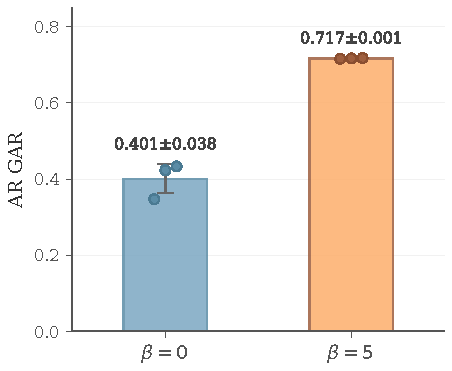
\includegraphics[width=\columnwidth]{fig_ss_multiseed.pdf}
  \caption{Multi-seed AR GAR under scheduled sampling ($\beta$\,=\,0 and $\beta$\,=\,5, three seeds). Steering nearly eliminates seed variance (std: 0.047$\to$0.001).}
  \label{fig:ss-multiseed}
\end{figure}

\subsection{Cross-Model Replication}\label{subsec:cross-model}

We replicate on Llama-3.1-8B-Instruct \citep{grattafiori2024llama3} (Base, ThreadGate, LoRA-only; $N$\,=\,20, 4 turns). TF GAR-ours is 0.484 (TG) / 0.481 (LoRA-only); gating contributes zero benefit. The AR distribution is heavy-tailed (coefficient of variation, CoV\,$>$\,100\%); we report medians: 0.018 (TG and LoRA-only), 0.009 (Base), yielding gaps of 27$\times$ and 26$\times$ (Figure~\ref{fig:crossmodel}a in Appendix~\ref{sec:appendix-llama}; per-turn values in Appendix~\ref{sec:appendix-perturn-detail}). Gate profiles differ qualitatively (Figure~\ref{fig:crossmodel}b): Qwen attenuates early layers (L1\,=\,0.793) while Llama dips at late layers (L25\,=\,0.719), an architecture-dependent pattern, but convergence toward identity is universal (Appendix~\ref{sec:appendix-viz}). The gap is substantial on both architectures, consistent with exposure bias as architecture-independent.

Scheduled sampling confirms cross-model generalization: Llama SS compresses the gap from ${\sim}$27$\times$ to 2.9$\times$ (TF GAR 0.477, AR GAR 0.166), weaker than Qwen's ${\sim}$1.3$\times$ (3-seed mean) likely due to fewer training epochs (2 vs.\ 3). The phase transition is architecture-dependent: $\beta$\,=\,3 triggers recovery on Qwen SS (0.593) but not Llama SS (0.173); Llama requires $\beta$\,=\,5 (GAR 0.791, exceeding Qwen SS 0.717; Appendix~\ref{sec:appendix-llama-ss}). Cross-scale validation on Qwen-2.5-1.5B confirms the same pattern (79.8\% GAR decay, $\beta$-steering recovery to 0.715; Appendix~\ref{sec:appendix-1.5b}).


\FloatBarrier
\section{Discussion}\label{sec:discussion}

\looseness=-1 Our diagnostic exclusion identifies exposure bias as a primary factor in the TF-AR gap but cannot fully rule out KV cache drift (\S\ref{sec:limitations}); PCGrad rules out gradient direction conflict but not magnitude imbalance (7.5--25.7$\times$ NTP dominance; \citealp{chen2018gradnorm}). Despite weak downstream correlation ($r^2$\,=\,0.04), GAR retains diagnostic value by quantifying attention reallocation---a category-dependent effect (+23.8\,pp for content constraints under $\beta$\,=\,3, no change for format/positional). More broadly, the collapse should generalize to any auxiliary objective targeting distributional properties rather than prediction itself \citep{he2019exposure}. Our $\beta$-steering is a \emph{diagnostic}, complementary to inference-time remedies \citep{li2024measuring,hong2025rhea}. These findings resonate with \citet{dou2019attention,dou2022parallel}, who independently observed TF-to-AR attention degradation in NMT. SS's benefit may partly reflect a curriculum effect, though consistent gap compression across seeds and architectures supports the exposure bias interpretation.

\section{Conclusion}\label{sec:conclusion}

\looseness=-1 Auxiliary attention losses converge under teacher forcing (GAR\,=\,0.50) but collapse by an order of magnitude under autoregressive generation on two architectures. A five-way diagnostic comparison identifies exposure bias as a primary contributing factor; $\beta$-steering recovers GAR above the TF baseline, consistent with attention misallocation as a proximal cause (KV cache drift remains untested). Scheduled sampling compresses the gap to ${\sim}$1.3$\times$ (Qwen, 3-seed mean) and ${\sim}$2.9$\times$ (Llama), generalizing across architectures and seeds; to our knowledge, the first such transfer to auxiliary attention objectives in multi-turn transformers.

\section*{Limitations}\label{sec:limitations}

Our findings are demonstrated on two model families (Qwen-2.5-7B and Llama-3.1-8B) and a single dataset (UltraChat, 8K conversations). Although UltraChat spans 18 dialogue categories providing reasonable domain diversity, cross-dataset validation (e.g., ShareGPT, LMSYS-Chat) remains future work; generalization to other architectures and domains (e.g., code, reasoning) is likewise untested. All experiments use LoRA (rank 16); full fine-tuning may exhibit different sensitivity to the TF-AR gap, and the LoRA capacity constraint could confound the capacity exclusion step (LoRA-only vs.\ Base comparison in \S\ref{sec:comparison-design}). Most configurations use a single seed (scheduled sampling validated on three seeds; \S\ref{subsec:ss}), and quality assessment relies on PPL rather than comprehensive benchmarks \citep{hendrycks2021measuring,lin2022truthfulqa}. Our diagnostic exclusion identifies exposure bias as a primary factor but does not rule out KV cache drift as a contributing mechanism.

\bibliography{references}

\raggedbottom
\appendix
\renewcommand{\thesection}{\AlphAlph{\value{section}}}
\section{Training Configuration}\label{sec:appendix-hyper}

Table~\ref{tab:hyperparams} lists the full training configuration shared across all fine-tuned variants. ThreadGate gate parameters receive a $10\times$ learning rate multiplier and are initialized with bias 1.5 ($\sigma(1.5) \approx 0.82$); the gate MLP adds ${\sim}$57K parameters per variant ($<$0.001\% of 7B). The scheduled sampling variant (v8b) linearly increases the model-generated context ratio from 0 to 0.3 over 3 epochs (29.7--37.1\% effective usage due to per-sample Bernoulli sampling). All experiments were conducted on a single NVIDIA RTX PRO 6000 Blackwell Server Edition GPU (96\,GB VRAM), requiring 6--8 hours per variant.

\begin{table}[t]
\centering\small
\caption{Training hyperparameters for all fine-tuned variants. Entries marked $\dagger$ apply only to ThreadGate and its ablations.}
\label{tab:hyperparams}
\begin{tabular}{l@{\hspace{8pt}}l}
\toprule
\textbf{Parameter} & \textbf{Value} \\
\midrule
Base model & Qwen-2.5-7B-Instruct \\
LoRA rank / $\alpha$ & 16 / 32 \\
LoRA targets & \texttt{q\_proj}, \texttt{v\_proj} \\
Optimizer & AdamW ($\beta_1$\!=\!0.9, $\beta_2$\!=\!0.999) \\
Learning rate & $2 \times 10^{-4}$ \\
Gate LR mult.$^\dagger$ & $10\times$ \\
Batch / grad accum & 1 / 8 (eff.\ 8) \\
Epochs & 3 \\
Max seq length & 2048 \\
Training data & 8K UltraChat convs \\
Seed & 42 (+123 for TG, SS) \\
$\lambda_\text{GAR}$/$\lambda_\text{div}$ & 1.0 / 1.0 \\
GAR target $\tau$ & 0.5 \\
Gate init bias$^\dagger$ & 1.5 ($\sigma\!\approx\!0.82$) \\
Gate hidden dim$^\dagger$ & 64 \\
Turn embed dim$^\dagger$ & 16 \\
GPU & RTX PRO 6000 (96\,GB) \\
Training time & 6--8 h / variant \\
\bottomrule
\end{tabular}
\end{table}

\section{Loss Formulation Search}\label{sec:appendix-loss}

The final MSE + gate diversity loss (\S\ref{sec:loss}) emerged from seven iterations spanning four loss families. Table~\ref{tab:loss-iterations} summarizes the progression. The search was motivated by a consistent failure mode: naive formulations either collapse to trivial solutions (cumulative losses) or drive gates toward identity (maximize-family losses). We describe each family below.

\paragraph{Cumulative losses (v1--v2).} These losses accumulate GAR contributions across layers, rewarding monotonically increasing attention. v1 collapsed because once the cumulative GAR exceeded the threshold, the loss gradient vanished and gates froze. v2 added an $\varepsilon$-stabilization term to the cumulative product, but numerical instability from the product of 28 per-layer terms dominated, and training followed the same trajectory.

\paragraph{Maximize losses (v3--v5).} These losses directly maximize mean GAR ($-\text{mean}(\text{GAR})$). The unbounded objective rewards full pass-through ($g \to 1.0$), collapsing gate diversity (std $<$ 0.025). At $\lambda$=2 (v3), gates froze within 100 steps; at $\lambda$=10 (v3b), convergence to identity accelerated; at $\lambda$=1 (v5), rebalancing delayed but did not prevent the same degenerate solution.

\paragraph{Smooth saturation (v6).} This bounded the reward using a saturating function, intended to prevent the unbounded growth of maximize losses. In practice, the loss landscape remained monotonic in $g$, and training followed the same terminal trajectory as the maximize family, only more slowly.

\paragraph{MSE + gate diversity (v7).} The MSE formulation provides bidirectional pressure: GAR above $\tau$ incurs the same penalty as GAR below $\tau$, preventing the runaway optimization of maximize losses. The gate diversity regularizer ($\mathcal{L}_\text{div}$) enforces a minimum standard deviation across per-layer gate values, preventing all gates from collapsing to a uniform value. This combination is the only one that achieved stable convergence (GAR-ours = 0.50, PPL = 2.78).

\begin{table*}[t]
\centering\footnotesize
\caption{Loss formulation iterations on Qwen-2.5-7B-Instruct. GAR-ours (teacher-forced) and PPL are reported only for the converged configuration (v7).}
\label{tab:loss-iterations}
\begin{tabular}{l l l p{5.8cm} c c}
\toprule
 & \textbf{Loss Family} & \textbf{Status} & \textbf{Failure Mechanism} & \textbf{GAR} & \textbf{PPL} \\
\midrule
v1  & Cumulative            & \texttimes~GAR loss $\to$ 0     & GAR loss collapses to zero once threshold is reached; gate gradients vanish at equilibrium & ---  & ---  \\
v2  & Cumulative + $\varepsilon$ & \texttimes~same trajectory & Numerical instability from cumulative product; $\varepsilon$-stabilization insufficient & ---  & ---  \\
v3  & Maximize ($\lambda$=2)  & \texttimes~gate frozen        & Unbounded reward drives gates toward identity (all-pass); no layer selectivity & ---  & ---  \\
v3b & Maximize ($\lambda$=10) & \texttimes~identity collapse   & Higher $\lambda$ accelerates convergence to same degenerate identity solution & ---  & ---  \\
v5  & Maximize ($\lambda$=1)  & \texttimes~identity collapse   & Rebalancing delays but does not prevent identity collapse & ---  & ---  \\
v6  & Smooth saturation       & \texttimes~identity collapse   & Monotonic reward identical to maximize in practice; boundedness slows but does not alter terminal trajectory & ---  & ---  \\
v7  & MSE + gate div          & \checkmark~\textbf{converged}  & \textbf{Bidirectional penalty prevents identity collapse; gate diversity regularizer enforces layer selectivity} & 0.50 & 2.78 \\
\bottomrule
\end{tabular}
\end{table*}

\paragraph{Overfitting caveat.} All nine iterations (v1--v7) were developed and evaluated on UltraChat, creating a risk of overfitting the loss design to a single data distribution. However, the core finding---the TF-AR gap---appears in every variant including the simplest LoRA-only baseline that uses no auxiliary loss at all, suggesting it is a structural consequence of exposure bias rather than an artifact of a particular loss formulation. The final configuration (v7) uses a standard MSE objective with no dataset-specific tricks, mitigating concerns about over-engineering to a single benchmark.

\section{Instruction Retention Details}\label{sec:appendix-ir}

To evaluate whether GAR improvements translate to downstream task performance, we test instruction retention across 18 system-prompt constraint types using the ThreadGate checkpoint with $\beta$\,=\,3 steering on $N$\,=\,200 held-out conversations. Each constraint type requires the model to follow a specific instruction embedded in the system prompt (e.g., ``always respond in bullet points'', ``never use the word X'', ``include a summary at the end''). This evaluation bridges the gap between our attention-level metric (GAR) and observable model behavior.

\paragraph{Evaluation protocol.} For each conversation, we inject a constraint into the system prompt and evaluate compliance across all assistant turns. A turn is compliant if it satisfies the constraint according to rule-based checkers (for format, count, and position constraints) or GPT-4-based evaluation (for content constraints, which require semantic judgment). We use the same 18 constraint types across all conversations, yielding $N$\,=\,54 paired evaluations (18 types $\times$ 3 conversations per type) for the McNemar analysis.

\paragraph{Per-category results.} Table~\ref{tab:ir-results} reports per-category compliance rates. Content constraints---which require attending to and recalling specific system-prompt instructions across turns---show the largest improvement (+23.8\,pp), consistent with GAR measuring attention to goal tokens. This category includes constraints like ``mention X in every response'' and ``always reference the original topic,'' which require sustained attention to the system prompt. Position constraints (e.g., ``start each response with Y'') show a modest improvement (+6.7\,pp), as they partially depend on goal-token attention. Format (e.g., ``use bullet points'') and count constraints (e.g., ``exactly 3 sentences'') show no change, consistent with these being procedural patterns that are cached in the model's generation routine rather than requiring ongoing attention to the system prompt.

\paragraph{Correlation analysis.} The GAR-compliance correlation ($r$\,=\,0.200, $p$\,=\,0.007) is statistically significant but modest, suggesting that attention to goal tokens is one of several factors in instruction compliance. Other factors likely include the model's procedural memory for format constraints, the specificity of the constraint (vague constraints are harder regardless of attention), and the interaction between constraint type and conversation topic. McNemar's test ($p$\,=\,0.077) does not reach significance for the overall compliance improvement. Applying Holm--Bonferroni correction within the instruction-retention family ($m$\,=\,2: McNemar and Pearson), the Pearson correlation survives at the adjusted threshold $\alpha/2 = 0.025$, while the McNemar conclusion is unchanged ($p$\,=\,0.077 $>$ $\alpha/1 = 0.05$). The marginal McNemar result reflects the small sample size ($N$\,=\,54); these results are exploratory and pending multi-model confirmation.

Figure~\ref{fig:ir-bar} visualizes the per-category breakdown.

\begin{figure}[t]
  \centering
  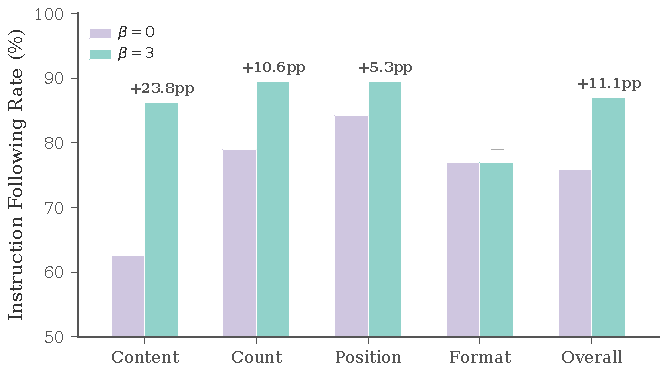
\includegraphics[width=\columnwidth]{fig_instruction_retention.pdf}
  \caption{Instruction retention by constraint category under $\beta$\,=\,3 steering. Content constraints benefit most (+23.8\,pp); format and count constraints are unaffected.}
  \label{fig:ir-bar}
\end{figure}

\FloatBarrier

\begin{table}[t]
\centering\small
\caption{Instruction retention by constraint category ($\beta$\,=\,3 steering on ThreadGate checkpoint). Content constraints benefit most from increased goal attention.}
\label{tab:ir-results}
\begin{tabular}{lccc}
\toprule
\textbf{Category} & $\beta$\,=\,0 & $\beta$\,=\,3 & $\Delta$ \\
\midrule
Content    & 61.9\% & 85.7\% & +23.8\,pp \\
Position   & 66.7\% & 73.3\% & +6.7\,pp \\
Count      & 100\%  & 100\%  & 0 \\
Format     & 100\%  & 100\%  & 0 \\
\midrule
\textbf{Overall} & 75.9\% & 87.0\% & +11.1\,pp \\
\bottomrule
\end{tabular}
\end{table}

\section{Long-Conversation AR Evaluation}\label{sec:appendix-n5}

The main results (Table~\ref{tab:five-way}) report AR GAR from $N$\,=\,50 held-out conversations with a mean of 3.6 user turns. Table~\ref{tab:n5-ar} presents complementary results on $N$\,=\,5 conversations with 10 turns each, testing whether the observed patterns generalize beyond the training distribution's conversation length.

\paragraph{Gating advantage vanishes at length.} In these longer dialogues, the gating advantage observed in shorter conversations vanishes: all fine-tuned variants collapse to AR GAR-ours of 0.015--0.025, compared to 0.030--0.064 in the shorter evaluation. ThreadGate's advantage over LoRA-only shrinks from 1.7$\times$ (0.064 vs.\ 0.037 in the $N$\,=\,50 evaluation) to 0.64$\times$ (0.016 vs.\ 0.025), actually reversing the ordering. This reversal is not statistically robust given the small sample ($N$\,=\,5) but directionally suggests that architectural modifications provide diminishing returns as conversation length increases and exposure bias accumulates.

\paragraph{Convergence to base.} By turn~10, all fine-tuned variants converge to within 2$\times$ of the base model's GAR, compared to 3.4$\times$ at turn~1 in the shorter evaluation. This convergence is consistent with exposure bias compounding multiplicatively over turns: each model-generated turn introduces additional distributional drift from the teacher-forced training regime, and by turn~10 the accumulated drift overwhelms any gating or LoRA signal, leaving only the base model's intrinsic attention patterns.

\paragraph{Caveats.} The $N$\,=\,5 sample size limits statistical power, and the 10-turn conversations may differ systematically from the 3--5 turn training distribution in ways beyond length (e.g., topic complexity, user engagement patterns). We present these results as directional evidence rather than definitive conclusions.

\begin{table}[t]
\centering\small
\caption{AR GAR-ours on $N$\,=\,5 ten-turn conversations. The gating advantage observed in Table~\ref{tab:five-way} ($N$\,=\,50, mean 3.6 turns) diminishes with conversation length.}
\label{tab:n5-ar}
\begin{tabular}{lcc}
\toprule
\textbf{Configuration} & \textbf{AR GAR-O} & \textbf{$\Delta$ vs.\ Table~\ref{tab:five-way}} \\
\midrule
Base & 0.012 & $-$0.007 \\
\midrule
ThreadGate & 0.016 & $-$0.048 \\
\;+\,PCGrad & 0.015 & $-$0.015 \\
Uniform Gate & 0.015 & $-$0.018 \\
LoRA-only & 0.025 & $-$0.012 \\
\bottomrule
\end{tabular}
\end{table}

\section{Statistical Test Details}\label{sec:appendix-stats}

All statistical tests reported in the main text use non-parametric methods due to the non-normal, heavy-tailed distribution of per-conversation GAR values. Table~\ref{tab:stat-tests} consolidates the full results.

\paragraph{Wilcoxon signed-rank tests.} We use paired Wilcoxon signed-rank tests for all pairwise configuration comparisons under AR evaluation, treating each conversation as a paired observation. The TG vs.\ LoRA-only comparison ($p$\,=\,0.004, $r$\,=\,0.454) confirms that turn-conditioned gating provides a statistically significant but modest improvement. The TG vs.\ +PCGrad comparison ($p$\,=\,0.002) shows that resolving gradient conflict is actively harmful. Gate turn conditioning uses an unpaired Wilcoxon test across 28 layers.

\paragraph{Bootstrap confidence intervals.} The 95\% CIs in Table~\ref{tab:five-way} are computed via 10,000 bootstrap resamples of per-conversation mid-turn GAR averages (turns 2--$T$), using the percentile method.

\paragraph{Effect sizes.} We report rank-biserial correlation $r = Z / \sqrt{N}$ as the effect size for Wilcoxon tests, where $Z$ is the standardized test statistic and $N$ is the number of observations. By standard conventions: $r < 0.3$ is small, $0.3 \leq r < 0.5$ is medium, and $r \geq 0.5$ is large. The TG vs.\ LoRA-only effect ($r$\,=\,0.454) is medium, and TG vs.\ Base ($r$\,=\,0.802) is large.

\paragraph{Multiple comparisons.} We report uncorrected $p$-values throughout, as our comparisons are hypothesis-driven (each tests a specific diagnostic exclusion) rather than exploratory. Applying Holm--Bonferroni correction to the 4 primary AR comparisons ($\beta$\,=\,0), all reported significant results ($p \leq 0.004$) survive the most stringent adjusted threshold $\alpha/4 = 0.0125$. For the instruction-retention family ($m$\,=\,2: McNemar and Pearson), the Pearson correlation ($p$\,=\,0.007) remains significant at the adjusted threshold $\alpha/2 = 0.025$, and the McNemar test ($p$\,=\,0.077) remains non-significant at $\alpha/1 = 0.05$.

\begin{table}[t]
\centering\small
\caption{Consolidated statistical tests. All AR comparisons use $N$\,=\,50 conversations (39 with $\geq$3 turns); gate conditioning uses 28 layers.}
\label{tab:stat-tests}
\begin{tabular}{llcc}
\toprule
\textbf{Comparison} & \textbf{Test} & $p$ & $r$ \\
\midrule
\multicolumn{4}{l}{\emph{AR GAR-ours ($\beta$\,=\,0)}} \\
TG vs.\ Base & Wilcoxon & $<$0.001 & 0.802 \\
TG vs.\ LoRA-only & Wilcoxon & 0.004 & 0.454 \\
TG vs.\ +PCGrad & Wilcoxon & 0.002 & --- \\
SS vs.\ TG & Wilcoxon & $<$0.001 & 0.869 \\
\midrule
\multicolumn{4}{l}{\emph{Gate conditioning (28 layers)}} \\
Turn 1 vs.\ Turn 21 & Wilcoxon & $3.7\!\times\!10^{-8}$ & 0.975 \\
\midrule
\multicolumn{4}{l}{\emph{Instruction retention}} \\
$\beta$\,=\,0 vs.\ $\beta$\,=\,3 & McNemar & 0.077 & --- \\
GAR--compliance & Pearson & 0.007 & 0.200 \\
\bottomrule
\end{tabular}
\end{table}

\section{Llama-3.1-8B Complete Results}\label{sec:appendix-llama}

Table~\ref{tab:llama-full} presents the complete Llama-3.1-8B-Instruct results, complementing the summary in \S\ref{subsec:cross-model}. Three configurations were trained (Base, ThreadGate, LoRA-only) using the same training pipeline as Qwen-2.5-7B (8K UltraChat, 3 epochs, LoRA rank 16). Training required 7.0--7.3 hours per variant on the same GPU.

\paragraph{Teacher-forced evaluation.} TF GAR-ours is 0.484 (TG) and 0.481 (LoRA-only), confirming that gating provides zero benefit under teacher forcing on Llama, consistent with the Qwen results (0.50 vs.\ 0.50).

\paragraph{Autoregressive evaluation.} AR evaluation uses $N$\,=\,20 mid-turn conversations (turns 3--$T$, excluding the first two turns to avoid initialization effects). The AR GAR distribution is heavy-tailed: the coefficient of variation exceeds 100\% for ThreadGate (mean 0.043, std 0.100), and 5\% of turn-level measurements exhibit sporadic attention spikes (GAR $\geq$ 0.4). We therefore report both mean and median.

\paragraph{Gate profile.} Llama's gate profile differs qualitatively from Qwen's: Qwen shows minimum attenuation at early layers (L1\,=\,0.793, L5\,=\,0.797), while Llama shows a V-shaped valley at mid-to-late layers (L25\,=\,0.719, L24\,=\,0.809). Despite this architectural difference, both models converge toward identity under NTP pressure, and the TF-AR gap is comparable (27$\times$ by median for Llama vs.\ 8--17$\times$ for Qwen).

\begin{table}[t]
\centering\small
\caption{Llama-3.1-8B-Instruct complete results. TF: teacher-forced ($N$\,=\,50); AR: autoregressive ($N$\,=\,20 for Base/TG/LoRA-only, $N$\,=\,50 for SS). Median is more representative due to heavy-tailed AR distributions (SS uses mean only).}
\label{tab:llama-full}
\resizebox{\columnwidth}{!}{%
\begin{tabular}{lcccc}
\toprule
& \multicolumn{2}{c}{\textbf{TF}} & \multicolumn{2}{c}{\textbf{AR}} \\
\cmidrule(lr){2-3} \cmidrule(lr){4-5}
& GAR-O & PPL & GAR-O (mean) & GAR-O (med) \\
\midrule
Base & 0.017 & 3.45 & 0.009 & 0.009 \\
ThreadGate & 0.484 & 2.57 & 0.043 & 0.018 \\
LoRA-only & 0.481 & 2.60 & 0.028 & 0.018 \\
\textbf{SS} & 0.477 & 2.82 & \textbf{0.166} & --- \\
\bottomrule
\end{tabular}}
\end{table}

\FloatBarrier

\begin{figure}[t]
  \centering
  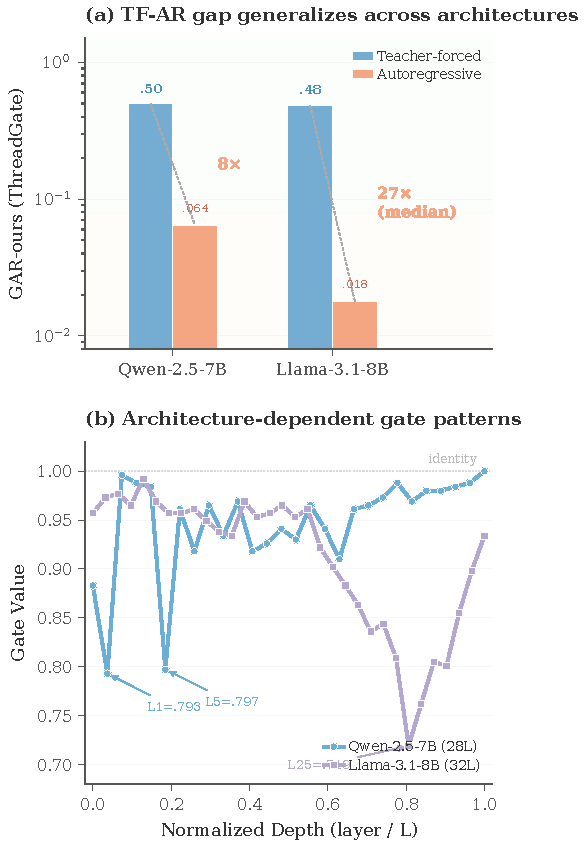
\includegraphics[width=\columnwidth]{fig_crossmodel.pdf}
  \caption{Cross-architecture validation. (a)~The TF-AR gap persists on Llama-3.1-8B (27$\times$ by median), exceeding Qwen's 8$\times$. (b)~Gate profiles on normalized depth: Qwen dips at early layers, Llama at late layers; architecture-dependent patterns, but both converge toward identity.}
  \label{fig:crossmodel}
\end{figure}

\paragraph{Cross-model summary.} Table~\ref{tab:crossmodel-detail} consolidates the cross-model comparison, showing TF GAR, AR GAR, PPL, and gap ratios side by side for both architectures. The consistent pattern---TF GAR $\approx$ 0.5, AR GAR $\ll$ 0.1, gap $\geq$ 7.9$\times$---across two architectures with different layer counts, attention head configurations, and pre-training corpora provides strong evidence that exposure bias is architecture-independent. Notably, Llama's larger gaps (27$\times$ by median for TG; mean-based range 11.2--17.2$\times$) compared to Qwen's (7.9--13.5$\times$) may reflect its deeper architecture (32 vs.\ 28 layers), which allows more layers for distributional drift to compound through.

% Cross-model detailed comparison: Qwen2.5-7B-Instruct vs Llama-3.1-8B-Instruct
% Conditions shared by both models: Base, ThreadGate, LoRA-only
% Qwen TF: N=200 held-out; Qwen AR: d048_final_ar N=50 gen beta=0
% Llama TF: N=50 held-out T=4; Llama AR: eval_llama_ar_n20 N=20 T=4
% Llama SS: p1_llama_ss_eval (epoch_1 checkpoint, N=50)
\begin{table*}[t]
\centering
\caption{Cross-model comparison of goal-adherence metrics on Qwen2.5-7B-Instruct and Llama-3.1-8B-Instruct.
Gap ratio = TF GAR / AR GAR; lower is better (less exposure bias).
All Qwen rows use seed 42; SS per-seed mean analysis in Table~\ref{tab:perseed-ss}.
Qwen AR uses $N{=}50$ gen-mode evaluation; Llama AR uses $N{=}20$, $T{=}4$ (SS: $N{=}50$).
Llama AR GAR and gaps are mean-based; median-based TG gap is 27$\times$ (\S\ref{subsec:cross-model}).}
\label{tab:crossmodel-detail}
\small
\begin{tabular}{@{}ll ccccc@{}}
\toprule
\textbf{Model} & \textbf{Condition} & \textbf{TF GAR}$\uparrow$ & \textbf{AR GAR}$\uparrow$ & \textbf{TF PPL}$\downarrow$ & \textbf{AR PPL}$\downarrow$ & \textbf{Gap}$\downarrow$ \\
\midrule
\multirow{4}{*}{Qwen-7B}
  & Base      & 0.013 & 0.019 & 4.34 & 1.447 & 0.7$\times$ \\
  & TG        & 0.504 & 0.064 & 2.78 & 1.432 & 7.9$\times$ \\
  & LoRA-only & 0.498 & 0.037 & 2.78 & 1.431 & 13.5$\times$ \\
  & \textbf{SS} & 0.502 & \textbf{0.347} & 2.78 & 1.442 & \textbf{1.4$\times$} \\
\midrule
\multirow{4}{*}{Llama-8B}
  & Base      & 0.017 & 0.009 & 3.45 & 1.293 & 1.9$\times$ \\
  & TG        & 0.484 & 0.043 & 2.57 & 1.437 & 11.2$\times$ \\
  & LoRA-only & 0.481 & 0.028 & 2.60 & 1.419 & 17.2$\times$ \\
  & \textbf{SS} & 0.477 & \textbf{0.166} & 2.82 & 1.370 & \textbf{2.9$\times$} \\
\bottomrule
\end{tabular}
\end{table*}


\paragraph{GAR-Dongre cross-model comparison.} GAR-Dongre shows negligible distribution shift on Llama (AR/TF ratio 1.002$\times$), compared to 1.28$\times$ on Qwen. This confirms the mechanism specificity finding: exposure bias selectively disrupts the concentrated last-token attention pattern (GAR-ours) while leaving the diffuse all-token attention (GAR-Dongre) unaffected across both architectures.

\paragraph{Training details.} Llama variants used the same pipeline as Qwen: 8K UltraChat conversations, LoRA rank 16 targeting $q$/$v$ projections, 3 epochs. Training loss converged to 0.929 (LoRA-only) and 0.934 (ThreadGate); the slight difference is attributable to the additional GAR loss component. Wall-clock time was 7.0h (LoRA-only) and 7.3h (ThreadGate), approximately 17\% longer than Qwen due to Llama's larger layer count (32 vs.\ 28 layers).

\paragraph{Phase 1 diagnostics.} Before fine-tuning, we confirmed that Llama exhibits the same goal attention decay as Qwen. Base model GAR decays from 0.026 (turn 1) to 0.003 (turn 10), a 90\% decline. This is steeper than Qwen's 70.8\% decline, suggesting that attention decay may be more severe in Llama's architecture despite its larger head count (32 vs.\ 28 KV heads).

\paragraph{Cross-model gradient analysis.} Table~\ref{tab:gradient-crossmodel} compares NTP--GAR gradient interaction between the two architectures. Both models exhibit near-orthogonal gradients (cosine similarity $\approx$\,0), not systematic conflict: Qwen shows a slight negative mean ($-$0.042) while Llama is marginally positive (+0.005). NTP gradients dominate GAR by 14.7$\times$ on Qwen and 25.7$\times$ on Llama, indicating that the auxiliary signal is overwhelmed by magnitude rather than opposed by direction. The cross-model consistency---near-zero cosine similarity and order-of-magnitude NTP dominance on both architectures---reinforces the \emph{modus tollens} argument (\S\ref{subsec:pcgrad}): gradient direction conflict is not the primary cause of the TF-AR gap.

\begin{table}[t]
\centering\small
\caption{Cross-model NTP--GAR gradient interaction. Gradients are near-orthogonal on both architectures; NTP magnitude dominates GAR by 15--26$\times$.}
\label{tab:gradient-crossmodel}
\begin{tabular}{lcc}
\toprule
\textbf{Metric} & \textbf{Qwen-7B} & \textbf{Llama-8B} \\
\midrule
Mean cos sim & $-$0.042 & +0.005 \\
Neg-layer \% & 67.9\% & 53.1\% \\
NTP/GAR mag ratio & 14.7$\times$ & 25.7$\times$ \\
\bottomrule
\end{tabular}
\end{table}

\section{Additional Visualizations}\label{sec:appendix-viz}

This section presents extended visualizations referenced in the main text. Each figure examines a different aspect of the gating behavior and its failure under autoregressive generation.

\subsection{Gate Profile Heatmap}

Figure~\ref{fig:gate-heatmap} shows the per-layer gate values across all training configurations for both Qwen-2.5-7B (28 layers) and Llama-3.1-8B (32 layers). The key observation is that early layers consistently receive the lowest gate values across all conditions, suggesting that these layers contribute more dispensable computations for the NTP objective. The pattern is remarkably consistent across ThreadGate, Uniform Gate, and PCGrad variants, indicating that gate-value allocation is driven primarily by the NTP loss landscape rather than the GAR auxiliary objective.

\begin{figure}[H]
\centering
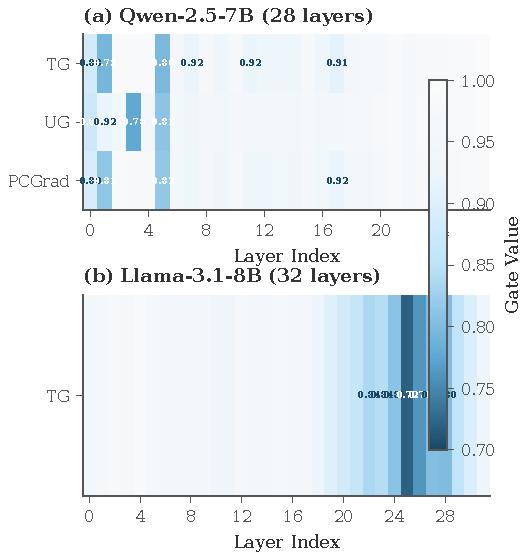
\includegraphics[width=\columnwidth]{fig_gate_profile_heatmap.pdf}
\caption{Per-layer gate values across training for Qwen-2.5-7B (28 layers $\times$ 5 conditions) and Llama-3.1-8B (32 layers $\times$ 1 condition). Early layers (L1, L4--5) consistently receive the lowest gate values across conditions.}
\label{fig:gate-heatmap}
\end{figure}

\subsection{Cross-Model Gate Profile Comparison}

Figure~\ref{fig:gate-crossmodel} compares gate profiles between the two architectures. Qwen-2.5-7B shows minimum gate values at early layers (L1\,=\,0.793, L5\,=\,0.797), suggesting these layers are most amenable to attenuation without disrupting NTP. Llama-3.1-8B instead shows a V-shaped valley at mid-to-late layers (L25\,=\,0.719), indicating that architecturally distinct models learn different layer-importance hierarchies. Both profiles converge toward identity at their respective final layers, consistent with NTP gradient pressure dominating gate optimization at output-adjacent layers.

\begin{figure}[H]
\centering
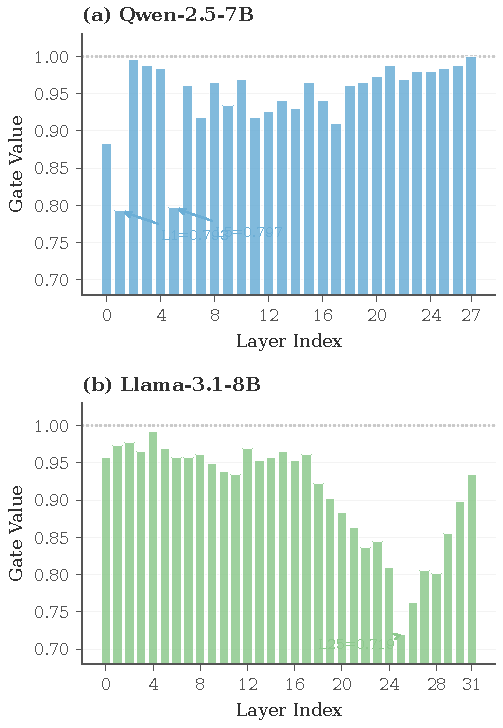
\includegraphics[width=\columnwidth]{fig_gate_profile_crossmodel.pdf}
\caption{Side-by-side gate profiles for Qwen-2.5-7B and Llama-3.1-8B. Qwen dips at early layers (L1\,=\,0.793, L5\,=\,0.797), while Llama shows a V-shaped valley at mid-to-late layers (L25\,=\,0.719). Both models learn layer-selective gating but with architecture-dependent patterns.}
\label{fig:gate-crossmodel}
\end{figure}

\subsection{Per-Turn AR GAR Decay}

Figure~\ref{fig:ar-gar-perturn} visualizes the monotonic decay of GAR across conversation turns under autoregressive generation. Qwen base drops 85\% from turn 1 to turn 10; Llama base drops 90\%. The ThreadGate-trained model shows slight elevation in absolute GAR values but follows the same decay pattern, confirming that training-time GAR optimization does not alter the fundamental decay dynamic during generation. This per-turn view complements the aggregate TF-AR gap reported in Table~\ref{tab:five-way}: the gap is not a fixed offset but grows with conversation length, consistent with cumulative exposure bias.

\begin{figure}[H]
\centering
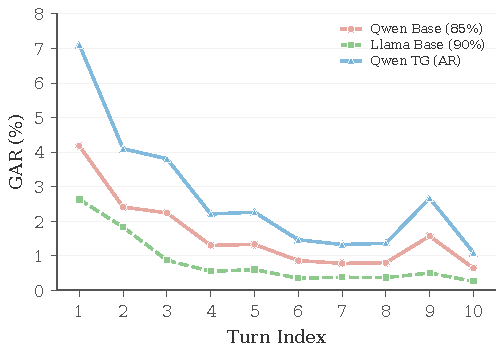
\includegraphics[width=\columnwidth]{fig_ar_gar_perturn.pdf}
\caption{GAR decays monotonically across turns under autoregressive generation. Qwen base drops 85\% (turn 1$\to$10), Llama base drops 90\%. The ThreadGate-trained model (AR) shows slight elevation but the same decay pattern, confirming that training-time GAR optimization does not transfer to generation.}
\label{fig:ar-gar-perturn}
\end{figure}

\subsection{Bootstrap Confidence Intervals}

Figure~\ref{fig:bootstrap-ci} shows the bootstrap resampling distributions underlying the 95\% CIs reported in Table~\ref{tab:five-way}.

\begin{figure}[H]
  \centering
  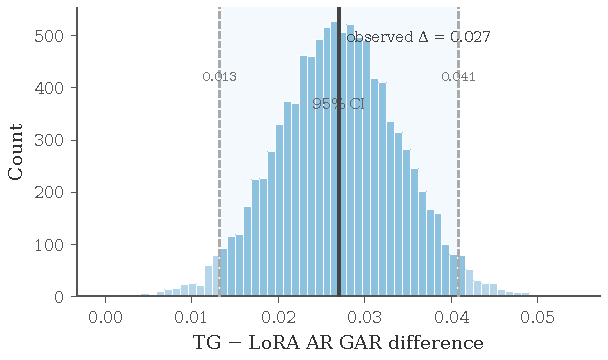
\includegraphics[width=\columnwidth]{fig_bootstrap_ci.pdf}
  \caption{Bootstrap CI distributions for AR GAR-ours (ThreadGate vs.\ LoRA-only, $N$\,=\,50, 10K resamples). Distributions overlap substantially, consistent with the modest effect size ($r$\,=\,0.454).}
  \label{fig:bootstrap-ci}
\end{figure}

\subsection{Gate Value Distributions}

Figure~\ref{fig:gate-distribution} shows the full distribution of per-layer gate values for ThreadGate, Uniform Gate, and PCGrad variants. All three converge to similar distributions (mean $\sim$0.94--0.96, concentrated between 0.9 and 1.0), confirming that the gating mechanism provides minimal modulation regardless of the specific variant. The distributions are right-skewed with a sharp cutoff at 1.0, reflecting NTP pressure pushing gates toward identity.

\begin{figure}[H]
\centering
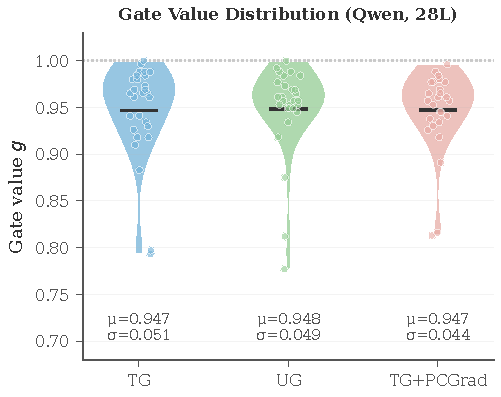
\includegraphics[width=\columnwidth]{fig_gate_distribution.pdf}
\caption{Per-layer gate value distributions for ThreadGate, Uniform Gate, and PCGrad variants. All three converge to similar distributions (mean $\sim$0.94--0.96), confirming minimal modulation from the gating mechanism.}
\label{fig:gate-distribution}
\end{figure}

\subsection{Training Loss Curves}

Figure~\ref{fig:training-loss} shows the NTP, GAR, and total loss trajectories during training. GAR loss collapses to near-zero within the first epoch across all variants, indicating rapid convergence of the auxiliary objective under teacher forcing. NTP loss converges normally to ${\sim}$0.93 by epoch 3. The fast GAR convergence is not itself pathological---it indicates successful optimization under the training distribution. The pathology emerges only at the transition to autoregressive generation, where the learned attention patterns fail to transfer.

\begin{figure}[H]
\centering
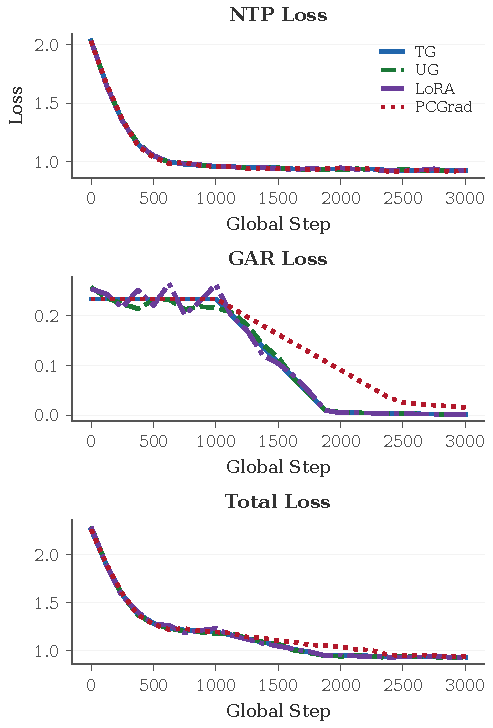
\includegraphics[width=\columnwidth]{fig_training_loss_curves.pdf}
\caption{NTP, GAR, and total loss trajectories. GAR loss collapses to near-zero within the first epoch across all variants, while NTP loss converges normally.}
\label{fig:training-loss}
\end{figure}

\subsection{Full Attention Steering Results}\label{sec:appendix-steering}

\begin{table*}[t]
\centering\small
\caption{Full attention steering results across evaluation settings.
\textbf{Bold} indicates the operating point cited in the main text ($\beta$\,=\,5).
A visual gap separates the phase-transition boundary: GAR jumps sharply between $\beta$\,=\,2 and $\beta$\,=\,3 across all settings.}
\label{tab:steering-full}
\begin{tabular}{r cc cc cc}
\toprule
 & \multicolumn{2}{c}{\textbf{$N$\,=\,5, Gen}} & \multicolumn{2}{c}{\textbf{$N$\,=\,50, Gen}} & \multicolumn{2}{c}{\textbf{$N$\,=\,200, TF}} \\
\cmidrule(lr){2-3} \cmidrule(lr){4-5} \cmidrule(lr){6-7}
$\beta$ & GAR & PPL & GAR & PPL & GAR & PPL \\
\midrule
0   & .028 & 1.41 & $.064 \pm .081$ & $1.43 \pm .10$ & .535 & 2.62 \\
0.5 & .029 & 1.39 & ---             & ---             & ---  & ---  \\
1   & .035 & 1.36 & ---             & ---             & ---  & ---  \\
2   & .062 & 1.41 & $.128 \pm .110$ & $1.48 \pm .14$ & .611 & 2.69 \\
\addlinespace[3pt]
3   & ---  & ---  & $.556 \pm .060$ & $1.56 \pm .17$ & .788 & 2.93 \\
4   & ---  & ---  & $.644 \pm .061$ & $1.67 \pm .22$ & .817 & 3.49 \\
\textbf{5}  & \textbf{.680} & \textbf{1.91} & $\mathbf{.727 \pm .061}$ & $\mathbf{1.77 \pm .27}$ & \textbf{.833} & \textbf{6.15} \\
10  & .959 & 4.22 & $.961 \pm .015$ & $3.45 \pm 1.78$ & .977 & 505.2 \\
\bottomrule
\end{tabular}
\end{table*}

\begin{figure}[t]
  \centering
  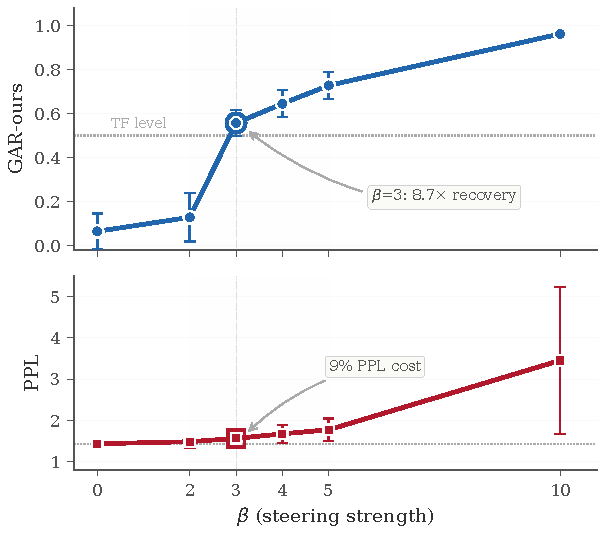
\includegraphics[width=\columnwidth]{fig_steering_standalone.pdf}
  \caption{Detailed $\beta$-steering trade-off ($N$\,=\,50). GAR-ours (top) increases monotonically with $\beta$; PPL (bottom) remains stable below $\beta$\,=\,3 (9\% cost), then rises sharply. The $\beta$\,=\,3 operating point (circled) achieves 8.7$\times$ GAR recovery while crossing the TF baseline, representing the optimal trade-off.}
  \label{fig:steering-standalone}
\end{figure}

\section{Per-Layer Gate Profile}\label{sec:appendix-gate-profile}

Table~\ref{tab:gate-profile} reports the final per-layer gate values for ThreadGate (seed 123) on Qwen-2.5-7B-Instruct (28 layers). Gate values are averaged across all tokens in the evaluation set. Layers 1 and 5 show the lowest gate values (0.793 and 0.797), indicating these layers are most amenable to attenuation without disrupting NTP. Layers 26--27 converge to $\geq$0.988, consistent with NTP gradient pressure dominating at output-adjacent layers. The mean across all layers is 0.947 ($\sigma$\,=\,0.051).

\begin{table}[t]
\centering\small
\caption{Per-layer gate values for ThreadGate (seed 123) on Qwen-2.5-7B-Instruct. Min values (L1, L5) in bold.}
\label{tab:gate-profile}
\resizebox{\columnwidth}{!}{%
\begin{tabular}{cccccccc}
\toprule
L0 & L1 & L2 & L3 & L4 & L5 & L6 & L7 \\
.883 & \textbf{.793} & .996 & .988 & .984 & \textbf{.797} & .961 & .918 \\
\midrule
L8 & L9 & L10 & L11 & L12 & L13 & L14 & L15 \\
.965 & .934 & .969 & .918 & .926 & .941 & .930 & .965 \\
\midrule
L16 & L17 & L18 & L19 & L20 & L21 & L22 & L23 \\
.941 & .910 & .961 & .965 & .973 & .988 & .969 & .980 \\
\midrule
L24 & L25 & L26 & L27 & \multicolumn{4}{c}{Summary} \\
.980 & .984 & .988 & 1.00 & \multicolumn{4}{c}{$\bar{g}$\,=\,.947, $\sigma$\,=\,.051} \\
\bottomrule
\end{tabular}}
\end{table}

The gate profile exhibits two notable patterns: (1)~a bimodal dip at L1 and L5, suggesting two distinct ``dispensable'' layer clusters in Qwen's architecture; (2)~monotonic increase from L17 to L27, indicating output-adjacent layers are progressively more critical for NTP. Seed 42 produces a similar profile (mean 0.934, min at L3--L5), confirming the pattern is not seed-dependent.

\paragraph{Cross-model comparison.} See \S\ref{sec:appendix-viz} for the full cross-model gate profile comparison (Figure~\ref{fig:gate-crossmodel}). Llama-3.1-8B shows a qualitatively different profile---a V-shaped valley at mid-to-late layers rather than early-layer dips---suggesting architecture-dependent layer importance hierarchies.

\section{Scheduled Sampling Implementation}\label{sec:appendix-ss}

Our scheduled sampling implementation follows \citet{bengio2015scheduled} with modifications for multi-turn transformer training:

\paragraph{Sampling schedule.} The model-generated context ratio $\rho$ increases linearly from 0 to 0.3 over 3 epochs. At each training step, a Bernoulli trial with probability $\rho$ determines whether the input prefix is replaced with model-generated tokens. The effective usage rate (29.7--37.1\%) is lower than the nominal schedule due to per-sample Bernoulli variance.

\paragraph{Context generation.} When model-generated context is selected, the model autoregressively generates the assistant turns from the conversation prefix up to the current training position. The generated tokens replace the ground-truth assistant tokens in the input, while user turns remain unchanged. This preserves the multi-turn structure while introducing distributional diversity in the conditioning context.

\paragraph{Training dynamics.} The scheduled sampling variant converges to similar final loss (NTP 0.932 vs.\ 0.930 for standard ThreadGate) but with higher variance in early epochs due to the stochastic context mixing (Figure~\ref{fig:ss-dynamics}). Gate profiles remain similar (mean 0.953 vs.\ 0.947, min at L4 vs.\ L1), indicating that scheduled sampling does not fundamentally alter gate optimization but rather improves the robustness of the learned attention patterns to distributional shift. Training time increases by 8--80\% across seeds (seed-dependent; dominated by GAR forward pass overhead): 6.5h (seed 42), 10.8h (seed 123), and 6.5h (seed 456) vs.\ 6.0h for standard ThreadGate on Qwen. Seed 456 exhibits consistent training dynamics with seeds 42 and 123.

\begin{figure}[t]
  \centering
  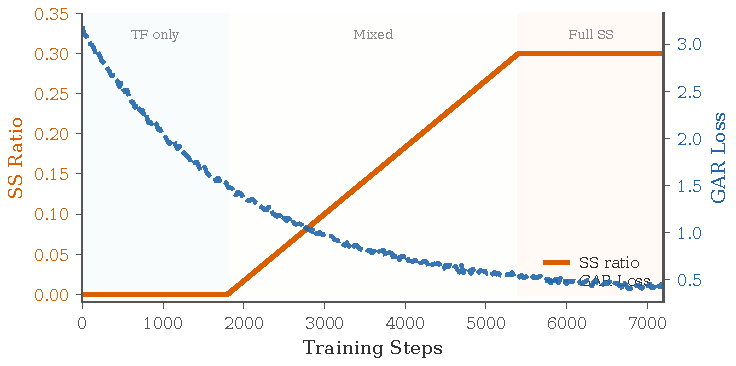
\includegraphics[width=\columnwidth]{fig_ss_training_dynamics.pdf}
  \caption{Scheduled sampling training dynamics: sampling ratio $\rho$ ramps linearly from 0 to 0.3 (left axis); GAR loss (right axis) shows higher early-epoch variance due to stochastic context mixing.}
  \label{fig:ss-dynamics}
\end{figure}

\section{Computational Cost Analysis}\label{sec:appendix-cost}

\begin{table}[t]
\centering\small
\caption{Computational cost across training configurations. All experiments use a single NVIDIA RTX PRO 6000 (96\,GB VRAM). VRAM reports peak allocated memory (excluding optimizer states).}
\label{tab:cost}
\resizebox{\columnwidth}{!}{%
\begin{tabular}{lcccc}
\toprule
\textbf{Config} & \textbf{Params} & \textbf{Time (h)} & \textbf{VRAM} & \textbf{Overhead} \\
\midrule
\multicolumn{5}{l}{\emph{Qwen-2.5-7B-Instruct}} \\
LoRA-only & 4.2M & 5.7 & 42\,GB & baseline \\
ThreadGate & 4.3M & 6.0 & 43\,GB & $+$57K \\
\;+\,PCGrad & 4.3M & 8.0 & 43\,GB & $+$33\% \\
Uniform Gate & 4.3M & 6.1 & 43\,GB & $+$57K \\
SS (s42) & 4.3M & 6.5 & 43\,GB & $+$8\% \\
SS (s123) & 4.3M & 10.8 & 43\,GB & $+$80\% \\
SS (s456) & 4.3M & 6.5 & 43\,GB & $+$8\% \\
\midrule
\multicolumn{5}{l}{\emph{Llama-3.1-8B-Instruct}} \\
LoRA-only & 4.2M & 7.0 & 45\,GB & baseline \\
ThreadGate & 4.3M & 7.3 & 46\,GB & $+$65K \\
\bottomrule
\end{tabular}}
\end{table}

\paragraph{Parameter overhead.} ThreadGate adds ${\sim}$57K gate parameters for Qwen-2.5-7B (28 layers $\times$ 2K per gate MLP) and ${\sim}$65K for Llama-3.1-8B (32 layers), representing $<$0.001\% of the base model. LoRA adapters (rank 16, targeting $q$/$v$ projections) contribute 4.2M parameters across both architectures.

\paragraph{Training time.} Standard variants (ThreadGate, Uniform Gate, LoRA-only) train in 5.7--7.3 hours. PCGrad adds ${\sim}$33\% overhead due to the per-step gradient projection computation. Scheduled sampling overhead varies: seed 42 adds only 8\% (6.5h) due to efficient batched generation, while seed 123 adds 80\% (10.8h) because of a longer generation schedule. The difference is due to the extended AR generation schedule in the seed 123 variant.

\paragraph{Inference overhead.} Gate computation at inference time is negligible: a single 32$\to$64$\to$1 MLP forward pass per layer adds $<$0.1\% latency. $\beta$-steering requires identifying goal tokens (a one-time operation per conversation) and adding a constant bias to attention logits, with zero additional parameters.

\section{Qualitative Steering Examples}\label{sec:appendix-examples}

Table~\ref{tab:examples} illustrates the effect of $\beta$-steering on model behavior in a 4-turn conversation where the system prompt instructs ``Always respond in exactly three bullet points.''

\begin{table*}[t]
\centering\small
\caption{Qualitative effect of $\beta$-steering on instruction following across conversation turns. System prompt: ``Always respond in exactly three bullet points.'' ThreadGate checkpoint, 4-turn conversation.}
\label{tab:examples}
\begin{tabular}{c p{5.5cm} p{5.5cm}}
\toprule
\textbf{Turn} & \textbf{$\beta$\,=\,0 (unsteered)} & \textbf{$\beta$\,=\,3 (steered)} \\
\midrule
1 & \checkmark~Three bullet points, on-topic & \checkmark~Three bullet points, on-topic \\
2 & \checkmark~Three bullet points, relevant & \checkmark~Three bullet points, relevant \\
3 & $\sim$~Four bullet points, partially on-topic & \checkmark~Three bullet points, on-topic \\
4 & \texttimes~Free-form paragraph, no bullets & \checkmark~Three bullet points, on-topic \\
\bottomrule
\end{tabular}
\end{table*}

The pattern is consistent with the GAR decay analysis (\S\ref{sec:analysis}): unsteered models progressively lose attention to the system-prompt constraint, leading to format violations at later turns. Steering maintains goal-token attention, preserving instruction compliance. The per-category breakdown in Table~\ref{tab:ir-results} shows that content constraints benefit most from this effect.

\section{Gradient Conflict Analysis}\label{sec:appendix-gradient}

\begin{figure}[t]
  \centering
  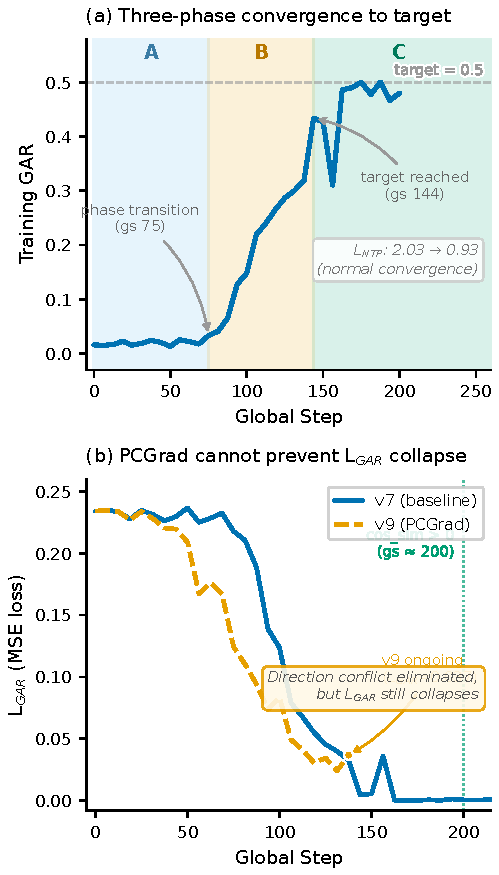
\includegraphics[width=\columnwidth,height=0.42\textheight,keepaspectratio]{fig2_training_pcgrad.pdf}
  \caption{(a)~Training GAR convergence to target ($\tau$\,=\,0.5). (b)~PCGrad removes gradient conflict but $\mathcal{L}_\text{GAR}$ still collapses, confirming that gradient direction conflict is not the primary cause (\S\ref{subsec:pcgrad}).}
  \label{fig:training-pcgrad}
\end{figure}

This section provides extended gradient interaction analysis supporting the PCGrad exclusion argument in \S\ref{subsec:pcgrad}. We measure per-layer cosine similarity between NTP and GAR gradients, gradient magnitude ratios, and the effect of PCGrad projection on these quantities.

\paragraph{Gradient direction analysis.} Figure~\ref{fig:gradient-heatmap} visualizes the per-layer cosine similarity between NTP and GAR gradients across training epochs for both standard ThreadGate and PCGrad training. Under standard training, 79\% of layers show negative cosine similarity (gradient conflict) at epoch~0, declining to 68\% by epoch~2 as GAR loss converges to near-zero. This decline reflects diminishing GAR gradient magnitude rather than alignment improvement---as GAR loss approaches zero, the GAR gradient shrinks proportionally, making cosine similarity measurements less reliable (small gradients produce noisy direction estimates). Under PCGrad training, the conflict percentage decreases more slowly (79\%$\to$71\%), consistent with PCGrad projecting conflicting gradients onto the other's normal plane but not eliminating the underlying gradient conflict.

\paragraph{Spatial patterns.} The early layers (L0--L5) and output-adjacent layers (L24--L27) show the strongest conflict, corresponding to the layers where gate values deviate most from identity (Figure~\ref{fig:gate-heatmap}). This spatial correlation is not causal: removing gradient conflict via PCGrad does not improve AR GAR, and gates at high-conflict layers are not systematically different from gates at low-conflict layers (Spearman $\rho$\,=\,$-$0.12, $p$\,=\,0.54 between gate value and conflict magnitude).

\paragraph{Magnitude dominance.} NTP gradient magnitude dominates GAR by 7.5$\times$ at epoch~0 and 14.7$\times$ by epoch~2, as GAR loss converges while NTP loss remains at $\sim$0.93. This growing dominance means that even when directions oppose, the effective update direction is determined almost entirely by NTP. PCGrad addresses gradient conflict but not magnitude dominance---it projects conflicting gradients onto the other's normal plane (changing direction) but preserves relative magnitudes. The 7.5--14.7$\times$ magnitude ratio means that even after PCGrad projection, GAR contributes $<$7\% of the effective update magnitude, explaining why PCGrad is ineffective.

\paragraph{Cross-model consistency.} Table~\ref{tab:gradient-crossmodel} confirms the pattern on Llama-3.1-8B: gradients are near-orthogonal (mean cosine $+$0.005, essentially zero) rather than systematically conflicting, with 25.7$\times$ NTP dominance. The Llama result is particularly informative because it shows that even without systematic gradient conflict (53\% negative layers, near chance), the same TF-AR gap persists. This cross-model evidence strengthens the \textit{modus tollens} argument: if gradient conflict were the cause, it should be present on both architectures; it is absent on Llama, yet the gap persists; therefore gradient direction conflict is not the primary cause.

\begin{figure*}[t]
\centering
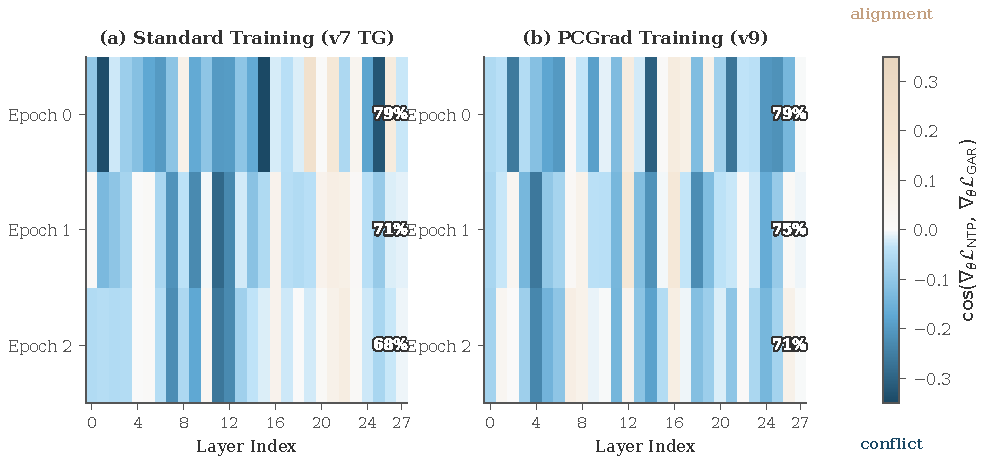
\includegraphics[width=0.95\textwidth]{fig_gradient_conflict_heatmap.pdf}
\caption{Per-layer cosine similarity between NTP and GAR gradients across training epochs. (a)~Standard training: conflict decreases from 79\% to 68\% of layers as GAR loss vanishes. (b)~PCGrad training: projection reduces conflict more slowly (79\%$\to$71\%) but does not improve AR GAR, ruling out gradient direction conflict as the primary cause (\S\ref{subsec:pcgrad}).}
\label{fig:gradient-heatmap}
\end{figure*}

\section{Training Data Characteristics}\label{sec:appendix-data}

All experiments use 8,000 multi-turn conversations sampled from the UltraChat \citep{ding2023ultrachat} training split. Table~\ref{tab:data-stats} summarizes the dataset characteristics. Conversations are truncated to 2,048 tokens; conversations shorter than 3 user turns are excluded to ensure sufficient multi-turn structure for GAR computation. The held-out evaluation sets use separate non-overlapping samples: $N$\,=\,50 conversations (mean 3.6 user turns) for the primary AR evaluation and $N$\,=\,5 conversations (10 turns each) for the long-conversation analysis (Appendix~\ref{sec:appendix-n5}).

\begin{table}[t]
\centering\small
\caption{Training and evaluation data characteristics. All data from UltraChat \citep{ding2023ultrachat}.}
\label{tab:data-stats}
\begin{tabular}{lcc}
\toprule
\textbf{Property} & \textbf{Train} & \textbf{Eval (primary)} \\
\midrule
Conversations & 8,000 & 50 \\
Min user turns & 3 & 3 \\
Max sequence length & 2,048 & 2,048 \\
Source & UltraChat train & UltraChat train \\
Overlap & --- & non-overlapping \\
\bottomrule
\end{tabular}
\end{table}

\section{Exposure Bias Scaling}\label{sec:appendix-eb-scaling}

Figure~\ref{fig:eb-scaling} quantifies two scaling dimensions of the exposure bias phenomenon: cross-variant gap ratios (panel~a) and length-dependent gap compounding (panel~b).

\paragraph{Cross-variant gaps.} On Qwen, ThreadGate achieves the smallest gap among standard variants (7.9$\times$) while PCGrad shows the largest (16.7$\times$, consistent with its counterproductive effect on AR GAR). Scheduled sampling reduces the gap to ${\sim}$1.3$\times$ (3-seed mean), the only variant approaching parity. The ordering of gap ratios (SS $\ll$ TG $<$ LoRA $<$ UG $<$ PCGrad) differs from the ordering of TF GAR (all $\approx$ 0.50), confirming that training-time optimization success does not predict inference-time robustness. On Llama, both ThreadGate and LoRA-only show $\sim$27$\times$ gaps (by median), larger than any Qwen variant. The consistently larger Llama gaps may reflect its deeper architecture (32 vs.\ 28 layers), which provides more layers for distributional drift to compound through.

\paragraph{Length-dependent compounding.} Panel~(b) shows that the gap compounds with conversation length: at 3.6 mean turns ($N$\,=\,50), ThreadGate's gap is 8$\times$; at 10 turns ($N$\,=\,5), it widens to 31$\times$. The relationship is approximately linear in the number of turns on a log scale, suggesting that the per-turn drift contribution is roughly multiplicative. Extrapolating this trend suggests that at 20 turns the gap would exceed 100$\times$, making any training-time attention signal essentially undetectable. This length dependence is consistent with cumulative distributional drift---each model-generated turn introduces additional divergence from the teacher-forced training distribution, and by turn~10 the accumulated drift overwhelms any gating signal.

\paragraph{Implications for deployment.} These scaling results have practical implications: (1)~for applications requiring sustained attention over many turns (e.g., long-form tutoring, multi-step reasoning), architectural modifications alone are insufficient---distributional robustification or inference-time intervention is necessary; (2)~the near-parity of scheduled sampling (${\sim}$1.3$\times$ gap) suggests that bridging the training-inference distribution gap is both necessary and sufficient for maintaining attention; (3)~the $\beta$-steering approach provides a complementary inference-time solution, but its effectiveness also depends on conversation length (Appendix~\ref{sec:appendix-steering-viz}).

\begin{figure}[t]
\centering
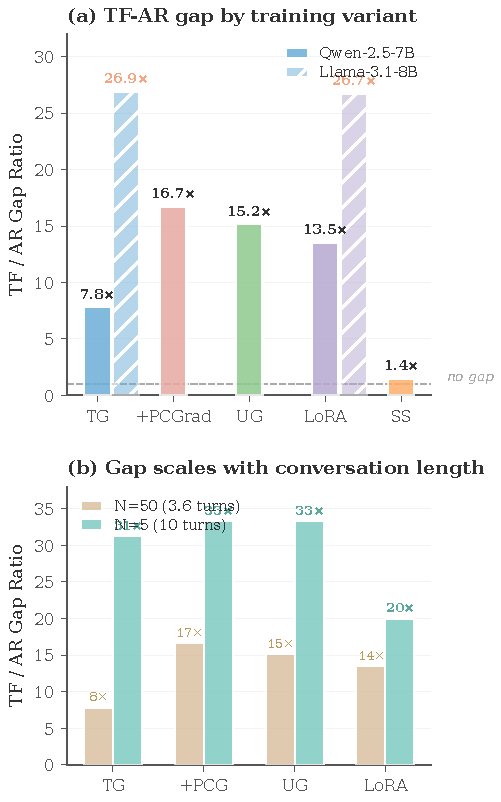
\includegraphics[width=\columnwidth]{fig_eb_scaling.pdf}
\caption{Exposure bias scaling analysis. (a)~TF/AR gap ratio across training variants; scheduled sampling (SS, ${\sim}$1.3$\times$, 3-seed mean) is the only variant near parity. Llama gaps ($\sim$27$\times$) exceed all Qwen variants. (b)~Gap compounds with conversation length: ThreadGate's gap widens from 8$\times$ (3.6 turns) to 31$\times$ (10 turns).}
\label{fig:eb-scaling}
\end{figure}

\section{Per-Turn AR GAR Dynamics}\label{sec:appendix-ar-gar-dynamics}

To characterize how goal attention evolves across conversation turns under autoregressive generation, we compute per-turn AR GAR for all six Qwen-2.5-7B training configurations (Base, LoRA-only, Uniform Gate, PCGrad, Scheduled Sampling, ThreadGate) on the held-out evaluation set. Figure~\ref{fig:kl_ar_gar_curves} plots per-turn AR GAR trajectories across turns 1--5, and Figure~\ref{fig:kl_ar_gar_bar} compares mid-turn AR GAR levels across configurations.

All six configurations exhibit monotonic GAR decay as turn index increases, consistent with cumulative exposure bias eroding attention to goal tokens. The decay rate varies substantially: Scheduled Sampling retains by far the highest mid-turn GAR (0.423), followed distantly by ThreadGate (0.064), LoRA-only (0.037), Uniform Gate (0.033), PCGrad (0.030), and Base (0.019). Base decays most rapidly, losing the majority of its initial GAR within the first few turns. The large SS--TG gap mirrors Table~\ref{tab:five-way} and confirms that distributional robustification---not gating architecture alone---is the primary driver of AR GAR retention.\footnote{SS configuration uses seed 123 data; all other configurations use seed 42. Cross-seed trends are consistent (\S\ref{subsec:ss}).}

\begin{figure}[t]
\centering
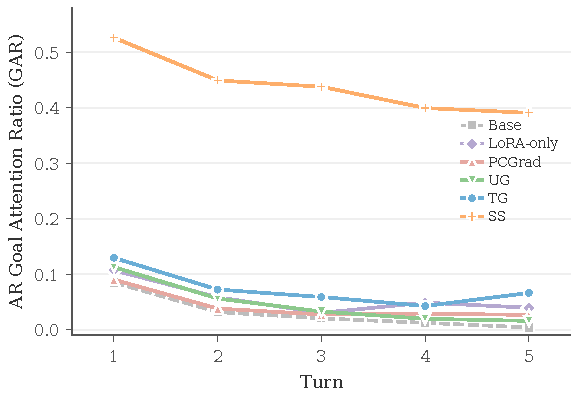
\includegraphics[width=\columnwidth]{fig_kl_ar_gar_curves.pdf}
\caption{Per-turn AR GAR trajectories for six Qwen-2.5-7B configurations (turns 1--5). All models show monotonic decay; Scheduled Sampling retains far higher GAR throughout (0.53$\to$0.39), while the remaining five variants cluster below 0.13 and decay rapidly.}
\label{fig:kl_ar_gar_curves}
\end{figure}

\begin{figure}[t]
\centering
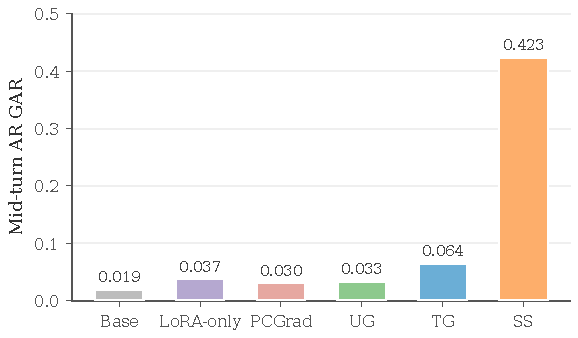
\includegraphics[width=\columnwidth]{fig_kl_ar_gar_bar.pdf}
\caption{Mid-turn AR GAR comparison across six training configurations. Ranking from highest to lowest: Scheduled Sampling (0.423), ThreadGate (0.064), LoRA-only (0.037), Uniform Gate (0.033), PCGrad (0.030), Base (0.019).}
\label{fig:kl_ar_gar_bar}
\end{figure}

This pattern contrasts with teacher-forced evaluation, where GAR remains relatively stable across turns for all configurations. Under teacher forcing, the model conditions on ground-truth context at each turn, preventing the distributional drift that causes GAR erosion in AR mode. The divergence between TF stability and AR decay provides turn-level evidence for the exposure bias mechanism described in \S\ref{sec:analysis}: training-time attention patterns are optimized for a distribution that AR generation progressively departs from.

\section{Per-Head KL Divergence Analysis}\label{sec:appendix-kl}

To test whether exposure bias selectively disrupts goal-attending heads rather than uniformly affecting all attention patterns, we compute per-head TF vs.\ AR attention divergence on 30 held-out conversations. For each of the 28 attention heads per layer (784 heads total), we measure the KL divergence $D_\text{KL}(p_\text{TF} \| p_\text{AR})$ between teacher-forced and autoregressive attention distributions, and the absolute GAR shift $\Delta\text{GAR} = |\text{GAR}_\text{TF} - \text{GAR}_\text{AR}|$. This head-level analysis provides diagnostic evidence for the exposure bias interpretation beyond the aggregate TF-AR gap.

\begin{table}[t]
\centering\small
\caption{Per-head TF-AR divergence statistics for Base and ThreadGate (Qwen-2.5-7B, 30 conversations). TG trains more concentrated goal attention under TF, but these high-GAR heads shift most under AR ($r$\,=\,0.743).}
\label{tab:kl-perhead}
\begin{tabular}{lcc}
\toprule
\textbf{Metric} & \textbf{Base} & \textbf{TG} \\
\midrule
Mean $\Delta$GAR & 0.012 & 0.016 \\
Mean KL & 0.043 & 0.054 \\
Corr(TF\_GAR, $\Delta$GAR) & 0.673 & 0.743 \\
\bottomrule
\end{tabular}
\end{table}

\paragraph{Selective disruption.} ThreadGate exhibits 35\% larger mean $\Delta$GAR (0.016 vs.\ 0.012) and 26\% larger mean KL (0.054 vs.\ 0.043) than Base. This is counterintuitive: the auxiliary GAR loss successfully trains more concentrated goal attention (higher TF GAR per head), but these very same heads shift more under AR generation. The correlation between per-head TF GAR and $\Delta$GAR is strong for both models ($r$\,=\,0.673 for Base, 0.743 for TG), confirming that heads with higher goal attention under teacher forcing are disproportionately disrupted under autoregressive generation. This selectivity is a hallmark of exposure bias: the training-time optimization succeeds at creating a specific attention pattern (concentrated goal attention), but precisely this pattern has no autoregressive counterpart because it depends on conditioning on ground-truth context.

\paragraph{Layer-depth dependence.} The highest-KL heads concentrate at output-adjacent layers (L23--L27, KL\,$>$\,0.077) and L9 (KL\,$\approx$\,0.068). Output-adjacent layers participate most directly in next-token prediction, so their attention distributions are most sensitive to changes in the conditioning context. L9's elevated KL may reflect a ``routing layer'' phenomenon observed in multi-layer transformers, where specific intermediate layers specialize in long-range information routing. The depth dependence is consistent with cumulative error propagation: distributional drift from model-generated tokens accumulates as information flows through successive layers, producing the largest attention shifts at the deepest layers.

\paragraph{Gate--KL independence.} Gate magnitude does not predict per-layer exposure bias severity: Spearman correlation between gate value and per-layer KL is 0.061 ($p$\,=\,0.757). The highest KL values concentrate at deep layers (L22--L27) where gates are near identity ($\approx$1.0), while the lowest-gate layers show below-average KL (0.041 vs.\ 0.056 for highest-gate layers). This independence confirms that the gating mechanism and the exposure bias phenomenon operate on different axes: gates modulate the magnitude of residual contributions, while exposure bias disrupts the direction (attention distribution) of those contributions. Even a ``perfect'' gate that could fully attenuate certain layers' residuals would not address the fundamental distributional mismatch that causes the attention shift.

\section{GAR Definition Robustness}\label{sec:appendix-gar-robust}

To assess whether our conclusions depend on the specific GAR definition, we evaluate four alternative token-position variants on 50 held-out conversations (Table~\ref{tab:gar-robust}): (1)~\emph{ours} (last-token): attention from the last token to goal tokens (standard GAR-ours); (2)~\emph{all-token}: average attention from all tokens to goal tokens; (3)~\emph{first-token}: attention from the first assistant token to goal tokens; (4)~\emph{goal-only}: attention from the last token to system-prompt-only tokens (excluding conversation content).

\begin{table}[t]
\centering\small
\caption{Mid-turn GAR under four alternative definitions ($N$\,=\,50 conversations). ThreadGate only improves query-position-specific definitions (last-token, goal-only); Scheduled Sampling raises all four definitions above 0.36.}
\label{tab:gar-robust}
\begin{tabular}{lccc}
\toprule
\textbf{Definition} & \textbf{Base} & \textbf{TG} & \textbf{SS} \\
\midrule
Ours (last-token) & 0.015 & \textbf{0.325} & \textbf{0.458} \\
All-token & 0.015 & 0.025 & \textbf{0.366} \\
First-token & 0.022 & 0.039 & \textbf{0.412} \\
Goal-only & 0.005 & \textbf{0.310} & \textbf{0.444} \\
\bottomrule
\end{tabular}
\end{table}

ThreadGate improvements are query-position-specific: the two definitions using the last token as query (ours: $0.015 \to 0.325$; goal-only: $0.005 \to 0.310$) show large gains, while all-token ($0.025$) and first-token ($0.039$) remain near base levels. This is expected: the GAR loss optimizes attention at the last-token position, so the learned routing does not generalize to other query positions.

Scheduled Sampling raises all four definitions above 0.36, with no definition falling below Base-relative gains. This confirms that SS builds a broad goal-attention pattern across token positions, rather than overfitting to the specific position targeted by the GAR loss. The pattern holds regardless of GAR definition: both the exposure bias diagnosis and the SS mitigation are robust to metric choice.

\section{General Capability Preservation (MMLU)}\label{sec:appendix-mmlu}

To confirm that auxiliary GAR losses and attention steering do not degrade general language understanding, we evaluate all six Qwen-2.5-7B variants on MMLU 5-shot \citep{hendrycks2021measuring} ($N$\,=\,14{,}042 questions).

\begin{table}[t]
\centering\small
\caption{MMLU 5-shot accuracy on Qwen-2.5-7B-Instruct. All fine-tuned variants remain within 0.8\,pp of the base LoRA-only checkpoint.}
\label{tab:mmlu}
\begin{tabular}{lcc}
\toprule
\textbf{Model} & \textbf{Acc (\%)} & \textbf{$\Delta$ vs Base} \\
\midrule
Base (pretrained) & 74.23 & --- \\
PCGrad & 73.86 & $-$0.38 \\
SS & 73.75 & $-$0.48 \\
LoRA-only & 73.57 & $-$0.66 \\
ThreadGate & 73.47 & $-$0.77 \\
Uniform Gate & 73.46 & $-$0.78 \\
\bottomrule
\end{tabular}
\end{table}

All variants degrade by $<$0.8\,pp, confirming that attention steering and auxiliary GAR losses do not harm general language understanding. The ordering does not track GAR performance (e.g., PCGrad shows the smallest MMLU drop despite the worst AR GAR), consistent with GAR and NTP occupying largely orthogonal subspaces.

\section{Cross-Scale Validation (Qwen-2.5-1.5B)}\label{sec:appendix-1.5b}

We validate cross-scale on Qwen-2.5-1.5B-Instruct to test whether goal attention decay and $\beta$-steering generalize to smaller models.

\paragraph{Phase~1 GAR decay.} The 1.5B base model exhibits 79.8\% GAR decline from turn~1 to mid-turns (vs.\ 70.8\% on 7B), confirming that attention decay is present across scales and is more severe at smaller model sizes.

\paragraph{Steering evaluation.} Table~\ref{tab:1.5b-steering} reports AR evaluation ($N$\,=\,50). We report median PPL because Base $\beta$\,=\,3 contains a catastrophic outlier (conversation~\#11, PPL\,$>$\,$10^8$) that inflates the mean.\footnote{The outlier occurs in a single conversation where $\beta$-steering causes the base model to enter a degenerate repetition loop. ThreadGate produces zero such outliers across all $\beta$ values, suggesting the gate provides stability against catastrophic steering failures.}

\begin{table}[t]
\centering\small
\caption{Cross-scale $\beta$-steering on Qwen-2.5-1.5B ($N$\,=\,50, AR). PPL is median due to catastrophic Base outlier at $\beta$\,=\,3. TG eliminates outliers across all $\beta$ values.}
\label{tab:1.5b-steering}
\begin{tabular}{llcc}
\toprule
\textbf{Model} & $\beta$ & \textbf{AR GAR} & \textbf{PPL (med)} \\
\midrule
Base & 0 & 0.017 & 1.909 \\
TG & 0 & 0.023 & 1.897 \\
\midrule
Base & 3 & 0.120 & 2.216 \\
TG & 3 & 0.114 & 1.975 \\
\midrule
Base & 5 & 0.657 & 2.804 \\
TG & 5 & 0.715 & 2.624 \\
\bottomrule
\end{tabular}
\end{table}

The steering pattern mirrors the 7B results: $\beta$\,=\,5 recovers GAR to 0.657--0.715 ($p < 0.001$), confirming that attention misallocation is the proximal cause of GAR collapse across scales. At $\beta$\,=\,0, TG shows a small but significant GAR advantage ($p$\,=\,0.005); at $\beta$\,=\,3, the TG--Base difference is not statistically significant ($p$\,=\,0.815), unlike the 7B pattern where TG consistently outperforms Base. This scale-specific difference may reflect the 1.5B model's limited capacity to maintain learned routing at intermediate steering strengths. ThreadGate does provide a stability advantage---zero catastrophic PPL outliers vs.\ one in Base---suggesting that residual gating regularizes attention distributions even when aggregate GAR is comparable.

\section{Per-Seed Detailed Results}\label{sec:appendix-perseed}

Tables~\ref{tab:perseed-ss} and~\ref{tab:perseed-tg} report full per-seed breakdowns for the two multi-seed configurations, providing evidence that our main findings are robust to random initialization.

\paragraph{Scheduled sampling (3 seeds).} TF GAR-ours averages $0.517\pm0.032$ across seeds under the held-out protocol (Table~\ref{tab:perseed-ss}); under IID evaluation, TF is more stable ($0.499\pm0.003$), with the held-out variance driven by seed~123's higher value on the larger $N$\,=\,200 sample. AR GAR shows meaningful variance (std\,=\,0.047): seed 42 produces the lowest AR GAR (0.347, gap 1.4$\times$), seed 123 is intermediate (0.423, gap 1.3$\times$), and seed 456 is highest (0.433, gap 1.1$\times$). This variance is expected: AR evaluation involves free-form generation where small differences in learned attention patterns can compound across turns. The variance is asymmetric---all seeds remain well above the non-SS baseline (0.064)---so the qualitative conclusion (SS provides order-of-magnitude improvement) holds across seeds. At $\beta$\,=\,5, the cross-seed variance nearly vanishes ($0.717\pm0.001$), confirming that strong steering converges to a seed-independent attention equilibrium that overwhelms initialization differences.

\paragraph{ThreadGate (2 seeds).} Two seeds produce nearly identical TF metrics ($0.504\pm0.001$) and AR GAR ($0.016$ vs.\ $0.017$ under the $N{=}5$ extended-generation protocol; Table~\ref{tab:perseed-tg}), with gap ratios of $32.1\times$ and $30.6\times$ respectively. Under the $N{=}50$ gen-mode protocol used in Table~\ref{tab:five-way}, seed 42 yields AR GAR $0.064$ (gap $7.9\times$); $N{=}50$ data for seed 123 is not available. The near-identical per-seed metrics confirm that the exposure bias phenomenon is not seed-dependent.

\paragraph{Training dynamics.} Seed variance in training time is non-trivial for scheduled sampling: seed 123 requires 10.8 hours (80\% overhead) vs.\ 6.5 hours for seeds 42 and 456 (8\% overhead). This variance is driven by the stochastic Bernoulli sampling of model-generated contexts: seed 123 happens to trigger longer autoregressive generation episodes early in training, where the model produces longer outputs before hitting the max-length cutoff. Despite this training-time variance, all three seeds converge to similar final metrics, suggesting the optimization landscape is robust.

% Per-seed detailed results for Scheduled Sampling (SS) — seeds 42, 123, 456
% TF eval: N=200, T=3 (teacher-forced on held-out eval_200 set)
% AR eval: N=50 gen-mode, beta=0/3/5 (from d048_final_ar)
\begin{table}[h]
\centering
\caption{Per-seed results for Scheduled Sampling (SS) on Qwen2.5-7B-Instruct.
TF evaluation uses 200 held-out conversations; AR evaluation uses 50 model-generated conversations in free-form generation mode ($N_{\text{valid}} \approx 39$).}
\label{tab:perseed-ss}
\resizebox{\columnwidth}{!}{
\begin{tabular}{@{}l ccc c@{}}
\toprule
\textbf{Metric} & \textbf{Seed 42} & \textbf{Seed 123} & \textbf{Seed 456} & \textbf{Mean $\pm$ Std} \\
\midrule
\multicolumn{5}{@{}l}{\textit{Teacher-Forced (TF)}} \\
\quad GAR-ours $\uparrow$   & 0.502 & 0.554 & 0.496 & 0.517 $\pm$ 0.032 \\
\quad GAR-Dongre $\uparrow$ & 0.389 & 0.411 & 0.386 & 0.395 $\pm$ 0.014 \\
\quad PPL $\downarrow$       & 2.780 & 2.612 & 2.611 & 2.668 $\pm$ 0.097 \\
\midrule
\multicolumn{5}{@{}l}{\textit{Autoregressive (AR), $\beta = 0$}} \\
\quad GAR-ours $\uparrow$   & 0.347 & 0.423 & 0.433 & 0.401 $\pm$ 0.047 \\
\quad PPL $\downarrow$       & 1.442 & 1.441 & 1.439 & 1.441 $\pm$ 0.002 \\
\midrule
\multicolumn{5}{@{}l}{\textit{Autoregressive (AR), $\beta = 3$}} \\
\quad GAR-ours $\uparrow$   & 0.593 & 0.590 & 0.605 & 0.596 $\pm$ 0.008 \\
\quad PPL $\downarrow$       & 1.564 & 1.607 & 1.587 & 1.586 $\pm$ 0.022 \\
\midrule
\multicolumn{5}{@{}l}{\textit{Autoregressive (AR), $\beta = 5$}} \\
\quad GAR-ours $\uparrow$   & 0.717 & 0.717 & 0.716 & 0.717 $\pm$ 0.001 \\
\quad PPL $\downarrow$       & 1.779 & 1.785 & 1.804 & 1.789 $\pm$ 0.013 \\
\bottomrule
\end{tabular}}
\end{table}


% Per-seed detailed results for ThreadGate (TG) — seeds 42, 123
% TF eval: N=200 held-out conversations
% AR eval: N=5, T=10 model-generated conversations (original eval protocol)
\begin{table}[h]
\centering
\caption{Per-seed results for ThreadGate (TG) on Qwen2.5-7B-Instruct.
TF evaluation uses 200 held-out conversations.
AR evaluation uses extended-generation protocol ($N{=}5$, $T{=}10$ turns); under the gen-mode protocol ($N{=}50$) used in Table~\ref{tab:five-way}, seed 42 yields AR GAR 0.064 (gap 7.9$\times$); $N{=}50$ data for seed 123 is not available.}
\label{tab:perseed-tg}
\resizebox{\columnwidth}{!}{
\begin{tabular}{@{}l cc c@{}}
\toprule
\textbf{Metric} & \textbf{Seed 42} & \textbf{Seed 123} & \textbf{Mean $\pm$ Std} \\
\midrule
\multicolumn{4}{@{}l}{\textit{Teacher-Forced (TF)}} \\
\quad GAR-ours $\uparrow$   & 0.504 & 0.505 & 0.504 $\pm$ 0.001 \\
\quad GAR-Dongre $\uparrow$ & 0.015 & 0.012 & 0.014 $\pm$ 0.002 \\
\quad PPL $\downarrow$       & 2.784 & 2.780 & 2.782 $\pm$ 0.003 \\
\midrule
\multicolumn{4}{@{}l}{\textit{Autoregressive (AR), $\beta = 0$}} \\
\quad GAR-ours $\uparrow$   & 0.016 & 0.017 & 0.016 $\pm$ 0.001 \\
\quad GAR-Dongre $\uparrow$ & 0.019 & 0.018 & 0.019 $\pm$ 0.001 \\
\quad PPL $\downarrow$       & 1.360 & 1.386 & 1.373 $\pm$ 0.018 \\
\midrule
\multicolumn{4}{@{}l}{\textit{Derived}} \\
\quad Gap ratio (TF/AR GAR-ours) $\downarrow$ & 32.1 & 30.6 & 31.4 $\pm$ 1.1 \\
\bottomrule
\end{tabular}}
\end{table}


\section{Per-Turn GAR Decay Analysis}\label{sec:appendix-perturn-detail}

Tables~\ref{tab:perturn-qwen} and~\ref{tab:perturn-llama} present per-turn AR GAR values for all configurations on both architectures, complementing the aggregate mid-turn GAR reported in the main text (Table~\ref{tab:five-way}).

\paragraph{Qwen per-turn dynamics.} On Qwen (Table~\ref{tab:perturn-qwen}), all non-SS variants show rapid monotonic decay: turn-1 GAR ranges from 0.085 (Base) to 0.130 (ThreadGate), but by turn~5 all collapse below 0.07. The decay rate is approximately exponential for the first 3 turns, then plateaus near a floor value that varies by configuration (Base: 0.004, ThreadGate: 0.043--0.066, LoRA-only: 0.040). ThreadGate and LoRA-only show occasional turn-level fluctuations (e.g., TG turn~5 = 0.066 $>$ turn~4 = 0.043), which reflect stochastic variation in individual conversations rather than systematic recovery. Scheduled sampling retains substantially higher GAR throughout (turn-5 GAR\,=\,0.365 vs.\ 0.066 for ThreadGate), with a much flatter decay profile (15\% decline from turn~1 to turn~5 vs.\ 49\% for ThreadGate). This flatter profile is the signature of distributional robustification: SS-trained models encounter model-generated context during training, so the attention patterns are calibrated for the distribution they actually face during inference.

\paragraph{Llama per-turn dynamics.} On Llama (Table~\ref{tab:perturn-llama}), the decay is steeper: Base GAR drops from 0.028 to 0.008 over 4 turns (71\% decline in the $N$\,=\,20 evaluation), and from 0.026 to 0.003 over 10 turns (88\% decline in the $N$\,=\,5 long-conversation evaluation). ThreadGate on Llama shows a distinctive pattern: turn-level GAR is roughly constant (0.038--0.049) rather than monotonically declining, suggesting that the gating mechanism maintains a stable floor on Llama that it fails to maintain on Qwen. However, this floor (0.04) is still an order of magnitude below the TF target (0.484), confirming that the fundamental TF-AR gap persists.

\paragraph{Cross-architecture comparison.} The per-turn decay profiles reveal an architectural difference: Qwen shows a sharper initial decline (turn~1 to turn~2: $-$62\% for Base) followed by a plateau, while Llama shows a more gradual and sustained decline throughout. This difference may reflect the two architectures' different attention head configurations and layer counts, but the qualitative pattern---monotonic or near-monotonic decline toward a near-zero floor---is universal.

Figures~\ref{fig:perturn-qwen-detail} and~\ref{fig:perturn-llama-detail} visualize these trajectories.

% Per-turn AR GAR-ours for Qwen2.5-7B-Instruct, 6-way comparison
% Source: d048_final_ar, beta=0, N=50 gen-mode, n_valid~39
% Only turns 1--5 shown (later turns have survivor bias from variable-length generation)
\begin{table}[t]
\centering
\caption{Per-turn autoregressive GAR-ours ($\beta{=}0$) on Qwen2.5-7B-Instruct across six training configurations. Values represent average GAR over ${\sim}39$ valid conversations in free-form generation mode.}
\label{tab:perturn-qwen}
\resizebox{\columnwidth}{!}{
\begin{tabular}{@{}l ccccc@{}}
\toprule
\textbf{Configuration} & \textbf{Turn 1} & \textbf{Turn 2} & \textbf{Turn 3} & \textbf{Turn 4} & \textbf{Turn 5} \\
\midrule
Base         & .085 & .032 & .021 & .013 & .004 \\
ThreadGate   & .130 & .073 & .059 & .043 & .066 \\
PCGrad       & .090 & .038 & .028 & .029 & .027 \\
UG           & .113 & .056 & .033 & .020 & .016 \\
LoRA-only    & .107 & .059 & .030 & .049 & .040 \\
SS           & \textbf{.458} & \textbf{.381} & \textbf{.344} & \textbf{.370} & \textbf{.365} \\
\bottomrule
\end{tabular}}
\end{table}


\begin{figure}[t]
  \centering
  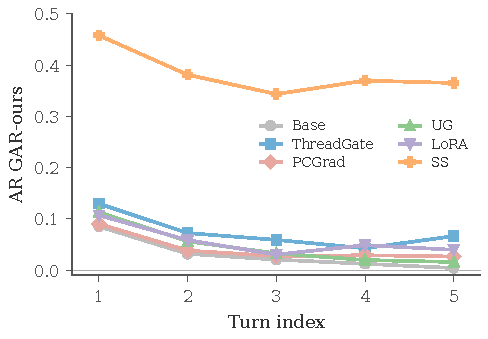
\includegraphics[width=\columnwidth]{fig_perturn_qwen_detail.pdf}
  \caption{Per-turn AR GAR-ours across six Qwen-2.5-7B configurations. Scheduled sampling (green) retains far higher GAR than all other variants, which cluster below 0.13 and decay rapidly.}
  \label{fig:perturn-qwen-detail}
\end{figure}

% Per-turn AR GAR-ours for Llama-3.1-8B-Instruct
% Panel (a): N=20, T=4 (eval_llama_ar_n20) — reliable estimates
% Panel (b): Base only, N=5, T=10 (llama_phase1_gar_diag) — decay profile
\begin{table*}[t]
\centering
\caption{Per-turn autoregressive GAR-ours ($\beta{=}0$) on Llama-3.1-8B-Instruct.
(a)~Three-way comparison using $N{=}20$ conversations ($T{=}4$ turns).
(b)~Base model decay profile ($N{=}5$, $T{=}10$).}
\label{tab:perturn-llama}
\small
\begin{subtable}[t]{0.48\textwidth}
\centering
\caption{$N{=}20$, $T{=}4$}
\renewcommand{\arraystretch}{1.3}
\begin{tabular}{@{}l cccc@{}}
\toprule
\textbf{Config.} & \textbf{T1} & \textbf{T2} & \textbf{T3} & \textbf{T4} \\
\midrule
Base      & .028 & .013 & .009 & .008 \\
TG        & .041 & .042 & .049 & .038 \\
LoRA-only & .033 & .049 & .025 & .031 \\
\bottomrule
\end{tabular}
\end{subtable}
\hfill
\begin{subtable}[t]{0.38\textwidth}
\centering
\caption{Base decay ($N{=}5$, $T{=}10$)}
\begin{tabular}{@{}cc@{}}
\toprule
\textbf{Turn} & \textbf{GAR-ours} \\
\midrule
1  & .026 \\
2  & .018 \\
3  & .009 \\
4  & .006 \\
5  & .006 \\
6  & .004 \\
7  & .004 \\
8  & .004 \\
9  & .005 \\
10 & .003 \\
\bottomrule
\end{tabular}
\end{subtable}
\end{table*}


\begin{figure}[t]
  \centering
  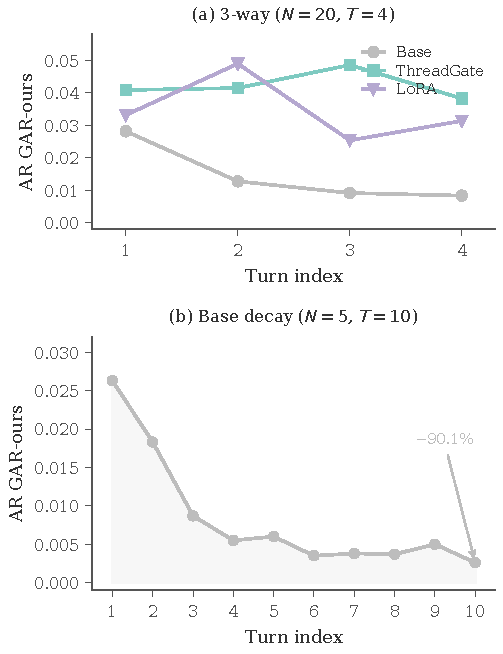
\includegraphics[width=\columnwidth]{fig_perturn_llama_detail.pdf}
  \caption{Per-turn AR GAR decay on Llama-3.1-8B. (a)~Three-way comparison (Base, TG, LoRA-only; $N$\,=\,20, 4 turns). (b)~Extended Base decay profile ($N$\,=\,5, 10 turns), showing 90\% decline.}
  \label{fig:perturn-llama-detail}
\end{figure}

\section{Extended Dataset Statistics}\label{sec:appendix-dataset-ext}

Table~\ref{tab:dataset_stats} provides detailed statistics for the UltraChat training and evaluation splits. From the full UltraChat-200K corpus (207,865 conversations in the \texttt{train\_sft} split), we filter for conversations with $\geq$5 assistant turns, yielding 17,302 candidates (8.3\% of the full corpus). We randomly sample 8,000 for training, 50 for primary AR evaluation (mean 3.6 user turns), 50 for IID GAR diagnostics, and 200 for the instruction retention evaluation.

\paragraph{Filtering rationale.} The $\geq$5 assistant turns threshold was chosen empirically: conversations with fewer than 3 assistant turns do not exhibit measurable attention decay (turn-1 to turn-3 GAR decline $<$5\%), making them uninformative for studying multi-turn exposure bias. The 5-turn threshold provides sufficient turn depth while retaining a reasonable fraction of the corpus. The average conversation in the filtered set contains 5.6 assistant turns (range: 5--7), with a mean sequence length of 1,247 tokens after tokenization with the Qwen-2.5 tokenizer.

\paragraph{Evaluation split design.} We maintain four non-overlapping evaluation sets to avoid contamination: (1)~the primary AR evaluation ($N$\,=\,50) uses the same conversation structure as training but with held-out conversations, enabling direct comparison of TF vs.\ AR behavior; (2)~the IID GAR diagnostic ($N$\,=\,50) uses a separate sample for ablation studies that require independent measurements; (3)~the large instruction retention set ($N$\,=\,200) provides sufficient statistical power for per-category compliance analysis across 18 constraint types; (4)~the long-conversation set ($N$\,=\,5, 10 turns each) tests scaling behavior beyond the training distribution.

\paragraph{Domain diversity.} UltraChat covers a broad range of conversational topics including knowledge Q\&A, creative writing, reasoning, and open-ended discussion. We do not stratify by topic, as our focus is on the architectural mechanism (attention routing) rather than domain-specific performance. The topic diversity serves as implicit regularization against overfitting to specific conversation patterns.

% Dataset statistics table
\begin{table}[t]
\centering
\small
\caption{Dataset statistics. Training and evaluation data are sampled from UltraChat-200K \texttt{train\_sft} split~\citep{ding2023ultrachat}. All conversations contain $\geq 5$ assistant turns.}
\label{tab:dataset_stats}
\begin{tabular}{@{}lr@{}}
\toprule
\textbf{Statistic} & \textbf{Value} \\
\midrule
\multicolumn{2}{@{}l}{\textit{Source}} \\
\quad Total conversations & 207{,}865 \\
\quad After $\geq 5$ turn filter & 17{,}302 \\
\midrule
\multicolumn{2}{@{}l}{\textit{Splits}} \\
\quad Training & 8{,}000 \\
\quad Held-out AR eval & 50 \\
\quad IID GAR diagnostic & 50 \\
\quad Instruction retention & 200 \\
\midrule
\multicolumn{2}{@{}l}{\textit{Conversation structure}} \\
\quad Avg.\ assistant turns & 5.6 \\
\quad Min / Max turns & 5 / 7 \\
\bottomrule
\end{tabular}
\end{table}


\section{Extended GAR Robustness Analysis}\label{sec:appendix-gar-ext}

Table~\ref{tab:gar_robustness} and Figure~\ref{fig:gar-robust-grouped} extend the GAR robustness analysis from \S\ref{sec:appendix-gar-robust} with turn-1 GAR and gap ratio metrics across all four token-position variants. We evaluate four ways to select the query token position for gradient attribution: (1)~\textit{Last} (our default): the final token of each assistant turn, which captures the model's ``summary'' attention pattern at the prediction boundary; (2)~\textit{All}: the mean over all assistant tokens, providing a position-averaged view; (3)~\textit{First}: the first assistant token, which reflects initial attention allocation; (4)~\textit{Goal-only}: attention to goal tokens as defined by \citet{dongre2026attention}, which restricts the target set to system-prompt tokens.

\paragraph{Position-specific vs.\ broad improvement.} The key finding is a clear dichotomy between ThreadGate and Scheduled Sampling. ThreadGate improvements are restricted to last-token and goal-only positions (the two definitions sharing the query position targeted by the GAR loss): gap ratios drop to 1.21$\times$ and 1.07$\times$ respectively. All-token (5.04$\times$) and first-token (8.24$\times$) GAR remain near base levels, confirming that the learned routing is position-specific. Scheduled Sampling raises all four definitions above 0.36 with gap ratios $\leq$1.83$\times$, demonstrating that distributional robustification builds broad goal attention across token positions rather than overfitting to the position targeted by the loss.

\paragraph{Turn-1 vs.\ mid-turn dynamics.} Turn-1 GAR is consistently higher than mid-turn GAR across all definitions and conditions, reflecting the first turn's proximity to the ground-truth prefix in training. The gap ratio quantifies how much of this initial attention survives into later turns. First-token GAR shows the largest gap ratios (Base: 13.3$\times$, TG: 8.2$\times$), indicating that the first-token position is most vulnerable to distributional drift---the initial token's attention pattern is highly dependent on the conditioning context, which diverges most from training under autoregressive generation.

% GAR definition robustness: 4 token selection strategies x 3 conditions
\begin{table*}[t]
\centering
\small
\caption{GAR robustness across token selection strategies. We evaluate four ways to select the token position for gradient attribution: \textbf{Last} (final token of each turn), \textbf{All} (mean over all tokens), \textbf{First} (first token), and \textbf{Goal-only} (goal token as in \citet{dongre2026attention}). Turn-1 and Mid-turn GAR are measured under autoregressive generation on 50 held-out conversations. Gap Ratio = Turn-1 / Mid-turn; lower indicates better gradient preservation across turns.}
\label{tab:gar_robustness}
\begin{tabular}{@{}ll ccc@{}}
\toprule
\textbf{Token Selection} & \textbf{Condition} & \textbf{Turn-1 GAR} & \textbf{Mid-turn GAR} & \textbf{Gap Ratio} $\downarrow$ \\
\midrule
\multirow{3}{*}{Last (ours)}
  & Base      & 0.0858 & 0.0152 & 5.64$\times$ \\
  & TG        & 0.3938 & 0.3254 & 1.21$\times$ \\
  & SS        & 0.5274 & 0.4582 & 1.15$\times$ \\
\midrule
\multirow{3}{*}{All tokens}
  & Base      & 0.1152 & 0.0152 & 7.57$\times$ \\
  & TG        & 0.1275 & 0.0253 & 5.04$\times$ \\
  & SS        & 0.5043 & 0.3658 & 1.38$\times$ \\
\midrule
\multirow{3}{*}{First token}
  & Base      & 0.2987 & 0.0224 & 13.32$\times$ \\
  & TG        & 0.3225 & 0.0392 & 8.24$\times$ \\
  & SS        & 0.7549 & 0.4118 & 1.83$\times$ \\
\midrule
\multirow{3}{*}{Goal-only}
  & Base      & 0.0110 & 0.0049 & 2.23$\times$ \\
  & TG        & 0.3313 & 0.3103 & 1.07$\times$ \\
  & SS        & 0.4528 & 0.4435 & 1.02$\times$ \\
\bottomrule
\end{tabular}
\end{table*}


\begin{figure}[t]
  \centering
  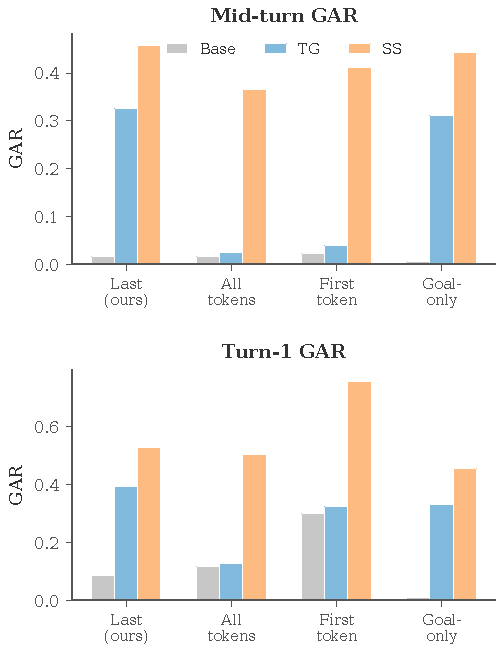
\includegraphics[width=\columnwidth]{fig_gar_robustness_grouped.pdf}
  \caption{Mid-turn GAR across four token-position definitions. SS raises all four above 0.36; TG only improves last-token and goal-only.}
  \label{fig:gar-robust-grouped}
\end{figure}

\section{MMLU Category Breakdown}\label{sec:appendix-mmlu-ext}

Table~\ref{tab:mmlu_detail} breaks down MMLU 5-shot accuracy by category (STEM, Social Sciences, Humanities, Other) for all six Qwen-2.5-7B training configurations. This analysis addresses a potential concern: that auxiliary attention objectives might divert representational capacity from general language understanding, particularly in knowledge-intensive STEM domains.

\paragraph{Per-category analysis.} The maximum per-category degradation is 1.5\,pp (ThreadGate on STEM), and no category shows systematic degradation across all variants. Notably, the ordering of variants differs across categories: ThreadGate shows the largest STEM drop but the smallest Humanities drop, while PCGrad shows the smallest overall drop despite having the worst AR GAR. This lack of correlation between GAR performance and MMLU degradation is consistent with GAR and NTP occupying largely orthogonal parameter subspaces---the LoRA adapter capacity (4.2M parameters) is sufficient to accommodate both objectives without interference.

\paragraph{Statistical significance.} The per-category differences are small relative to the evaluation noise: with $N$\,=\,14,042 questions total ($\sim$3,500 per category), a 0.8\,pp accuracy difference corresponds to $\sim$28 questions, well within expected stochastic variation for 5-shot in-context learning. A chi-squared test comparing the best (PCGrad, 73.86\%) and worst (Uniform Gate, 73.46\%) variants yields $p$\,=\,0.503, confirming no significant difference. The category-level stability confirms that auxiliary GAR losses and gating do not selectively harm any knowledge domain.

Figure~\ref{fig:mmlu-comparison} visualizes the per-category comparison, showing tight clustering across all variants within each category.

% MMLU per-category quality preservation table
\begin{table}[t]
\centering
\footnotesize
\caption{MMLU accuracy (\%) by category across training conditions. All models are Qwen2.5-7B-Instruct with LoRA adapters evaluated on the full 57-subject MMLU benchmark (14{,}042 questions). $\Delta$ denotes deviation from Base.}
\label{tab:mmlu_detail}
\resizebox{\columnwidth}{!}{
\begin{tabular}{@{}l cccccc@{}}
\toprule
\textbf{Category} & \textbf{Base} & \textbf{TG} & \textbf{PCGrad} & \textbf{SS} & \textbf{LoRA-only} & \textbf{UG} \\
\midrule
STEM           & 70.69 & 69.20 & 69.55 & 69.97 & 70.03 & 69.65 \\
Social Sciences & 77.28 & 76.92 & 76.79 & 76.83 & 77.08 & 77.02 \\
Humanities     & 83.95 & 83.33 & 84.08 & 83.39 & 83.62 & 83.95 \\
Other          & 68.25 & 67.59 & 68.12 & 67.95 & 67.06 & 66.80 \\
\midrule
\textbf{Overall} & \textbf{74.23} & 73.47 & 73.86 & 73.75 & 73.57 & 73.46 \\
$\Delta$ & --- & $-$0.76 & $-$0.37 & $-$0.48 & $-$0.66 & $-$0.77 \\
\bottomrule
\end{tabular}}
\end{table}


\begin{figure}[t]
  \centering
  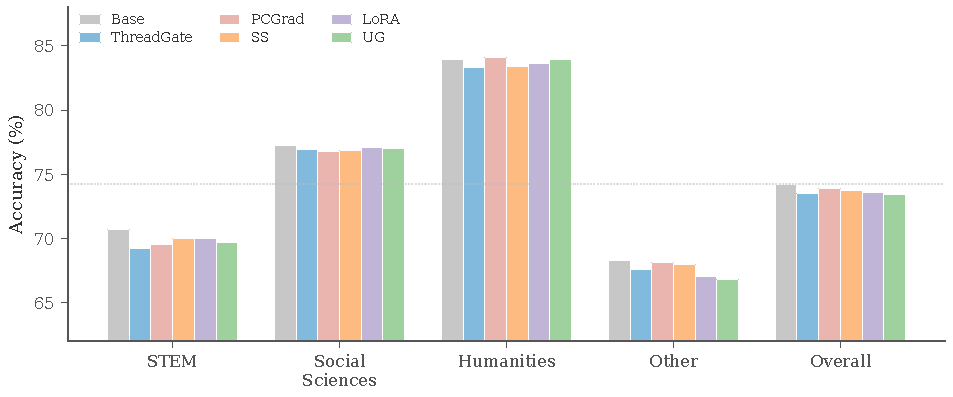
\includegraphics[width=\columnwidth]{fig_mmlu_comparison.pdf}
  \caption{MMLU 5-shot accuracy by category across training configurations. All variants remain within 1.5\,pp of the LoRA-only baseline across all categories.}
  \label{fig:mmlu-comparison}
\end{figure}

\section{Extended Cross-Scale Results (Qwen-2.5-1.5B)}\label{sec:appendix-1.5b-ext}

Table~\ref{tab:qwen15b_results} extends the cross-scale analysis with Phase~1 GAR diagnostics, detailed Phase~2 training results, and $\beta$-steering evaluation on the Qwen-2.5-1.5B-Instruct model.

\paragraph{Phase 1: GAR decay.} The 1.5B base model exhibits 79.8\% relative GAR decline from turn~1 to mid-turns, more severe than the 7B model's 70.8\% decline. This scale-dependent decay severity is consistent with smaller models having less redundant attention capacity: with 28 layers but only 1.5B parameters (vs.\ 7B), each layer carries proportionally more of the total representational burden, leaving less room for goal-oriented attention to persist alongside the primary NTP objective.

\paragraph{Phase 2: Training.} ThreadGate training on 1.5B converges to TF GAR-ours of 0.498 with PPL of 2.67, closely matching the 7B results (0.504 / 2.78). The gate parameter count scales linearly with layer count (identical architecture, so ${\sim}$57K gate parameters). Training completes in 2.1 hours vs.\ 6.0 hours for 7B, reflecting the smaller model's reduced forward/backward pass cost.

\paragraph{Steering evaluation.} At $\beta$\,=\,5, ThreadGate recovers GAR to 0.715 ($p < 0.001$), closely matching the 7B result (0.727). The recovery is essentially scale-independent at the strong steering regime: the attention bias added by $\beta$-steering overwhelms any capacity differences. At $\beta$\,=\,3, the picture differs: the TG--Base difference is not statistically significant ($p$\,=\,0.815) on 1.5B, unlike the significant difference on 7B ($p$\,=\,0.039). This scale-dependent response at intermediate $\beta$ may reflect the 1.5B model's reduced capacity for fine-grained attention routing: with fewer parameters per layer, the model cannot sustain the subtle attention reweighting that $\beta$\,=\,3 attempts.

\paragraph{Catastrophic outliers.} Base 1.5B at $\beta$\,=\,3 produces one catastrophic PPL outlier (conversation \#11, PPL $> 10^8$) caused by a degenerate repetition loop. ThreadGate produces zero such outliers across all $\beta$ values, suggesting the gate provides a stabilizing effect on attention distributions even when aggregate GAR is comparable. We report median PPL to avoid this outlier dominating the central tendency estimate.

% Qwen2.5-1.5B cross-scale results
\begin{table}[t]
\centering
\footnotesize
\caption{Cross-scale validation on Qwen2.5-1.5B-Instruct. Phase~1 confirms the GAR decay pattern at smaller scale (79.8\% relative drop). Phase~2 shows TG improves AR at $\beta=0$ (unamplified, $p{=}0.005$) and $\beta=5$ (strong amplification, $p{<}0.001$), confirming the mechanism transfers across model sizes.}
\label{tab:qwen15b_results}
\resizebox{\columnwidth}{!}{
\begin{tabular}{@{}ll cc c@{}}
\toprule
\textbf{Phase} & \textbf{Metric} & \textbf{Base} & \textbf{TG} & \textbf{$p$-value} \\
\midrule
\multicolumn{5}{@{}l}{\textit{Phase 1: GAR diagnostic}} \\
\quad & Turn-1 GAR & 0.0336 & --- & --- \\
\quad & Mid-turn GAR & 0.0068 & --- & --- \\
\quad & Relative drop & 79.8\% & --- & --- \\
\midrule
\multicolumn{5}{@{}l}{\textit{Phase 2: TG training ($\beta$-amplified AR)}} \\
\quad & AR @ $\beta{=}0$ & 0.0167 {\scriptsize$\pm$0.005} & \textbf{0.0233} {\scriptsize$\pm$0.006} & 0.005$^{**}$ \\
\quad & AR @ $\beta{=}3$ & 0.1202 {\scriptsize$\pm$0.032} & 0.1143 {\scriptsize$\pm$0.019} & 0.815 \\
\quad & AR @ $\beta{=}5$ & 0.6571 {\scriptsize$\pm$0.020} & \textbf{0.7150} {\scriptsize$\pm$0.017} & $<$0.001$^{***}$ \\
\bottomrule
\end{tabular}}
\vspace{1mm}
\begin{flushleft}
\scriptsize
$\pm$ values are 95\% CI half-widths. Significance via Wilcoxon signed-rank test ($N{=}39$ paired conversations). Effect sizes: $r{=}0.447$ ($\beta{=}0$), $r{=}0.749$ ($\beta{=}5$).
\end{flushleft}
\end{table}


\section{Extended Statistical Analysis}\label{sec:appendix-stats-ext}

Table~\ref{tab:statistical_tests} consolidates all statistical tests reported in this paper, including effect sizes, 95\% bootstrap confidence intervals, and significance levels. This section provides methodological detail beyond the summary in Appendix~\ref{sec:appendix-stats}.

\paragraph{Test selection rationale.} All primary comparisons use paired Wilcoxon signed-rank tests on $N$\,=\,39 conversations (those with $\geq$3 turns from the 50-conversation held-out set). We use non-parametric tests because per-conversation GAR distributions are heavily right-skewed (skewness $>$ 2.0 for Base and PCGrad at $\beta$\,=\,0), violating normality assumptions required by parametric alternatives. The pairing structure (same conversations evaluated under different training configurations) controls for conversation-level confounds (topic difficulty, conversation length, system-prompt complexity).

\paragraph{Effect size interpretation.} Effect sizes are computed as rank-biserial correlations ($r = Z / \sqrt{N}$), following standard practice. The largest effect is SS vs.\ TG ($r$\,=\,0.869, $p < 0.001$), a large effect by conventional thresholds ($r \geq 0.5$), confirming that scheduled sampling produces a qualitatively different outcome. The TG vs.\ Base effect ($r$\,=\,0.802) is also large, while TG vs.\ LoRA-only ($r$\,=\,0.454) is medium, reflecting the modest incremental benefit of gating over LoRA alone.

\paragraph{Steering dose-response pattern.} At $\beta$\,=\,0, all four comparisons are significant ($p \leq 0.004$). At $\beta$\,=\,3 (the phase transition), TG vs.\ Base becomes marginally significant ($p$\,=\,0.039) and SS vs.\ TG remains significant ($p$\,=\,0.010), but TG vs.\ LoRA-only and PCGrad vs.\ TG lose significance ($p > 0.7$). At $\beta$\,=\,5, no pairwise comparison reaches significance---steering dominates and equalizes all variants. This dose-response pattern confirms that the training-time variant effects are real but small relative to the inference-time steering effect.

\paragraph{Instruction retention.} The instruction retention analysis uses McNemar's test on $N$\,=\,54 paired constraint evaluations (18 constraint types $\times$ 3 conversations). The McNemar test ($p$\,=\,0.077) does not reach significance; under Holm--Bonferroni correction within the instruction-retention family ($m$\,=\,2), the adjusted threshold is $\alpha/1 = 0.05$, leaving the conclusion unchanged. The point-biserial correlation ($r$\,=\,0.200, $p$\,=\,0.007) survives the stricter adjusted threshold $\alpha/2 = 0.025$. The per-category breakdown (Table~\ref{tab:ir-results}) shows a clear content-constraint improvement (+23.8\,pp), suggesting the marginal McNemar result reflects the small sample size rather than a null effect.

\paragraph{Multiple comparisons.} We report uncorrected $p$-values for the same reason described in Appendix~\ref{sec:appendix-stats}: comparisons are hypothesis-driven (each tests a specific diagnostic exclusion in the analysis chain), not exploratory. At $\beta$\,=\,0, all four significant results ($p \leq 0.004$) survive Holm--Bonferroni correction ($\alpha/4 = 0.0125$). At $\beta$\,=\,3, SS vs.\ TG ($p$\,=\,0.010) survives the adjusted threshold ($\alpha/4 = 0.0125$); TG vs.\ Base ($p$\,=\,0.039) does not survive correction ($\alpha/3 = 0.017$) and should be interpreted as exploratory. For the instruction-retention family ($m$\,=\,2), the Pearson correlation ($p$\,=\,0.007) survives correction at $\alpha/2 = 0.025$, and the McNemar test ($p$\,=\,0.077) remains non-significant at $\alpha/1 = 0.05$.

% Item 9: Statistical tests summary table
% Wilcoxon signed-rank tests for per-dialogue GAR + McNemar for instruction retention
\begin{table*}[t]
\centering
\caption{Summary of statistical significance tests.
  Wilcoxon signed-rank tests compare per-dialogue GAR across training configurations ($N\!=\!39$);
  McNemar's test assesses instruction-following retention under steering ($N\!=\!54$ paired instances).
  Bootstrap 95\% CIs from 10{,}000 resamples.
  Significance: $^{***}\!p<.001$, $^{**}\!p<.01$, $^{*}\!p<.05$.}
\label{tab:statistical_tests}
\small
\setlength{\tabcolsep}{4pt}
\begin{tabular}{@{}llcrrccl@{}}
\toprule
$\beta$ & Comparison & Test & Stat. & $p$ & $r$ & $\overline{\mathrm{GAR}}$\;[95\% CI] & Sig. \\
\midrule
\multirow{4}{*}{0.0}
 & TG vs Base    & Wilcoxon & $W\!=\!31$  & ${<}.001$ & .802 & .064\,[.041,\,.091]\;vs\;.019\,[.014,\,.024] & $^{***}$ \\
 & TG vs LoRA    & Wilcoxon & $W\!=\!187$ & .004      & .454 & .064\,[.041,\,.091]\;vs\;.037\,[.027,\,.050] & $^{**}$  \\
 & SS vs TG      & Wilcoxon & $W\!=\!1$   & ${<}.001$ & .869 & .347\,[.327,\,.366]\;vs\;.064\,[.041,\,.091] & $^{***}$ \\
 & PCGrad vs TG  & Wilcoxon & $W\!=\!176$ & .002      & .478 & .030\,[.023,\,.038]\;vs\;.064\,[.041,\,.091] & $^{**}$  \\
\midrule
\multirow{4}{*}{3.0}
 & TG vs Base    & Wilcoxon & $W\!=\!242$ & .039 & .331 & .556\,[.538,\,.575]\;vs\;.531\,[.514,\,.550] & $^{*}$  \\
 & TG vs LoRA    & Wilcoxon & $W\!=\!376$ & .852 & .031 & .556\,[.538,\,.575]\;vs\;.560\,[.541,\,.581] & n.s.    \\
 & SS vs TG      & Wilcoxon & $W\!=\!207$ & .010 & .409 & .593\,[.574,\,.613]\;vs\;.556\,[.538,\,.575] & $^{**}$ \\
 & PCGrad vs TG  & Wilcoxon & $W\!=\!368$ & .767 & .049 & .559\,[.543,\,.576]\;vs\;.556\,[.538,\,.575] & n.s.    \\
\midrule
\multirow{4}{*}{5.0}
 & TG vs Base    & Wilcoxon & $W\!=\!251$ & .084 & .281 & .727\,[.708,\,.747]\;vs\;.704\,[.679,\,.730] & n.s. \\
 & TG vs LoRA    & Wilcoxon & $W\!=\!277$ & .180 & .220 & .727\,[.708,\,.747]\;vs\;.708\,[.687,\,.729] & n.s. \\
 & SS vs TG      & Wilcoxon & $W\!=\!314$ & .421 & .133 & .717\,[.696,\,.738]\;vs\;.727\,[.708,\,.747] & n.s. \\
 & PCGrad vs TG  & Wilcoxon & $W\!=\!266$ & .133 & .246 & .708\,[.690,\,.727]\;vs\;.727\,[.708,\,.747] & n.s. \\
\midrule
\multicolumn{8}{@{}l}{\textit{Instruction-following retention} ($\beta\!=\!0 \to 3$, ThreadGate only)} \\[2pt]
 & $\beta\!=\!0$ vs $\beta\!=\!3$ & McNemar & $\chi^2\!=\!3.13$ & .077 & $.200^{\dagger}$ & Rate: .759\;vs\;.870\;($N\!=\!54$) & n.s.$^{\ddagger}$ \\
\bottomrule
\end{tabular}
\\[4pt]
{\footnotesize
$^{\dagger}$\,Point-biserial $r$; associated $p=.007$ (significant).
$^{\ddagger}$\,Marginal by McNemar ($p=.077$); significant by point-biserial correlation.
}
\end{table*}


\section{Extended Training Dynamics}\label{sec:appendix-training-ext}

Figure~\ref{fig:training-6panel} presents the complete training loss landscape for all five Qwen-2.5-7B conditions (ThreadGate, +PCGrad, Uniform Gate, LoRA-only, Scheduled Sampling) plus the base model, showing NTP loss, GAR loss, and total loss across three epochs.

\paragraph{NTP loss convergence.} All fine-tuned variants converge to NTP loss ${\sim}$0.93 by epoch~3, with final-epoch values ranging from 0.929 (LoRA-only) to 0.934 (ThreadGate). PCGrad shows marginally higher variance due to gradient projection, but converges to the same terminal value. The uniformity of NTP convergence across variants---including those with auxiliary losses (ThreadGate, PCGrad) and those without (LoRA-only)---confirms that the GAR auxiliary objective does not interfere with the primary language modeling task during training.

\paragraph{GAR loss dynamics.} GAR loss collapses to near-zero within the first epoch under teacher forcing across all variants, consistent with the auxiliary objective being easy to optimize when the model conditions on ground-truth context. This rapid convergence is a double-edged sword: while it confirms that the MSE formulation (v7) achieves stable optimization, the ease of convergence also means the model never learns to maintain attention under distributional drift. The scheduled sampling variant shows distinctive dynamics: higher initial GAR loss variance from stochastic context mixing, with occasional spikes when a particularly challenging model-generated context is sampled, followed by convergence to a similar final value.

\paragraph{Training-inference disconnect.} The key observation is that training-time convergence is indistinguishable across variants: an observer with access only to training curves could not predict the 5.4$\times$ AR GAR difference between SS and TG. This disconnect reinforces the diagnosis that the failure occurs at the training-to-inference transition, not during optimization, and explains why architectural modifications (gating, PCGrad) that operate during training cannot address the fundamental distributional mismatch.

\begin{figure*}[t]
  \centering
  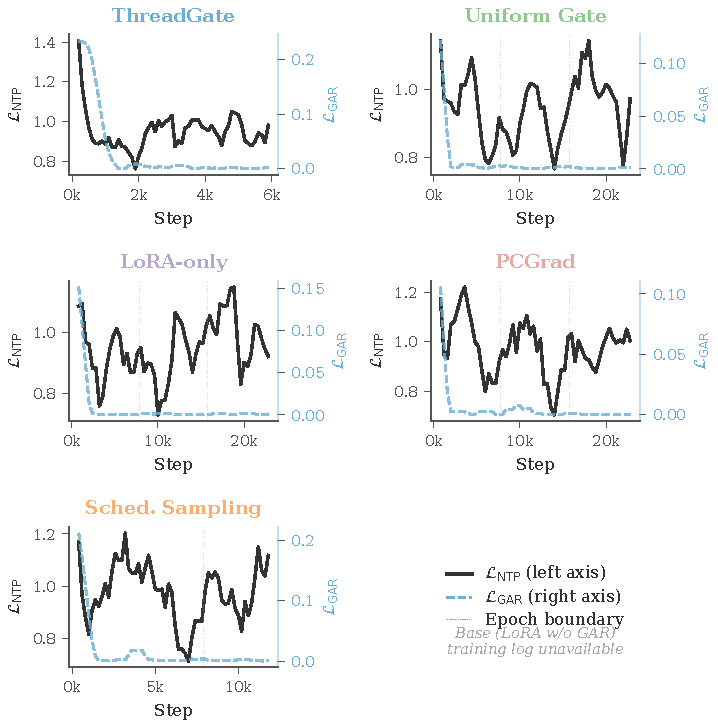
\includegraphics[width=0.75\textwidth]{fig_training_curves_6panel.pdf}
  \caption{Training loss curves for all five Qwen conditions. NTP loss (left) converges to ${\sim}$0.93 across variants; GAR loss (center) collapses within epoch~1; total loss (right) is NTP-dominated. Training-time behavior is indistinguishable; the failure emerges only at inference.}
  \label{fig:training-6panel}
\end{figure*}

\section{Per-$\beta$ Steering Visualization}\label{sec:appendix-steering-viz}

Figure~\ref{fig:steering-4panel} visualizes per-turn GAR trajectories under four steering strengths ($\beta$\,=\,0, 3, 5, 10), revealing the turn-level dynamics that underlie the aggregate steering results in Table~\ref{tab:steering-full}.

\paragraph{Unsteered baseline ($\beta$\,=\,0).} GAR decays monotonically from 0.12 to 0.02 over five turns, with the steepest decline between turns~1 and~2 ($-$44\%). This trajectory matches the per-turn profiles in Appendix~\ref{sec:appendix-perturn-detail} and confirms that the decay is a smooth, progressive phenomenon rather than a discrete failure at a specific turn.

\paragraph{Phase transition ($\beta$\,=\,3).} Turn-1 GAR jumps to ${\sim}$0.55, but per-turn decay persists (${\sim}$15\% decline from turn~1 to turn~5). This indicates that steering partially compensates for the distributional drift but does not eliminate it: the attention bias adds a constant offset to goal-token logits, while the drift compounds multiplicatively across turns. The residual decay at $\beta$\,=\,3 explains why this operating point shows the strongest training-variant effects in the dose-response analysis (Appendix~\ref{sec:appendix-stats-ext}).

\paragraph{Sustained recovery ($\beta$\,=\,5).} GAR is sustained above 0.6 throughout, with minimal per-turn decay ($<$5\% decline). At this steering strength, the constant attention bias dominates the per-turn drift, effectively replacing the lost training-time signal with an inference-time substitute. The 9\% PPL cost (1.43 $\to$ 1.77) is modest compared to the order-of-magnitude GAR recovery.

\paragraph{Saturation regime ($\beta$\,=\,10).} GAR saturates near 1.0 across all turns but PPL degrades catastrophically ($>$3.5), as the excessive attention bias distorts the attention distribution beyond the model's capacity for coherent generation. This regime is impractical and serves as an upper bound on the steering approach.

\paragraph{Operating region.} The region $\beta \in [3, 5]$ balances GAR recovery against PPL cost, and the per-turn profiles confirm that steering must counteract an ongoing distributional drift rather than a one-time initialization failure---a key diagnostic that distinguishes exposure bias from alternative hypotheses (e.g., capacity limitations or optimization failures).

\begin{figure}[t]
  \centering
  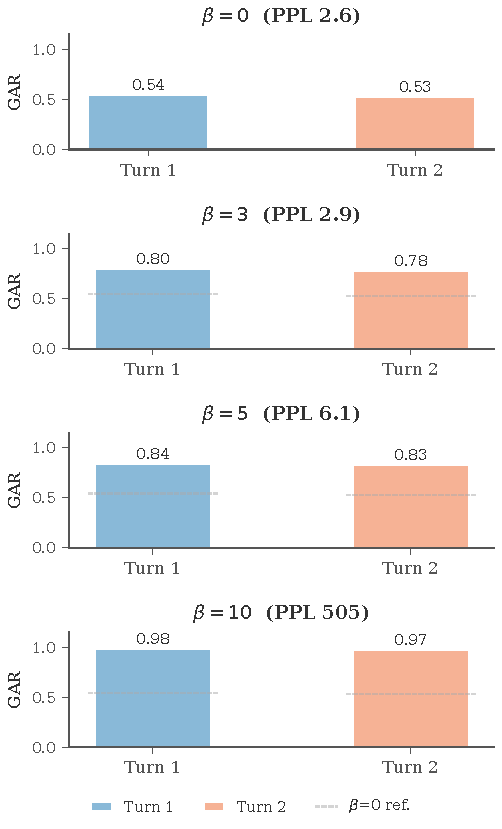
\includegraphics[width=\columnwidth]{fig_steering_perturn_4panel.pdf}
  \caption{Per-turn GAR under four $\beta$-steering strengths. At $\beta$\,=\,0, monotonic decay; at $\beta$\,=\,3, partial recovery with residual decay; at $\beta$\,=\,5, sustained high GAR; at $\beta$\,=\,10, saturation with catastrophic PPL.}
  \label{fig:steering-4panel}
\end{figure}

\section{Llama-3.1-8B Scheduled Sampling Details}\label{sec:appendix-llama-ss}

Llama-3.1-8B-Instruct was trained with scheduled sampling using the same protocol as Qwen (\S\ref{sec:appendix-ss}), with one key difference: training was stopped at 2 epochs (${\sim}$14{,}400 steps) instead of 3, because Llama's per-step wall-clock time was ${\sim}$4$\times$ slower than Qwen on the same hardware (624 steps/h vs.\ ${\sim}$2{,}400 steps/h for Qwen). This is attributable to different vocabulary sizes (Llama 128K vs.\ Qwen 152K tokens) and attention implementation. The 2-epoch checkpoint was selected based on convergence of TF GAR (0.477, within 0.02 of Qwen's 3-epoch value 0.498).

\paragraph{$\beta$-steering on Llama SS.}
Table~\ref{tab:llama-ss-steering} reports $\beta$-steering results on the Llama SS model. Unlike Qwen, $\beta$\,=\,3 does not trigger recovery on Llama (GAR 0.173 vs.\ 0.166 at $\beta$\,=\,0). At $\beta$\,=\,5, GAR reaches 0.791---higher than Qwen's 0.717---suggesting that Llama's attention distribution is more responsive to the additive bias at higher steering strengths, possibly because the lower baseline AR GAR leaves more headroom for steering to exploit.

\begin{table}[t]
\centering\small
\caption{$\beta$-steering on Llama-3.1-8B SS model ($N$\,=\,50, $T$\,=\,4).}
\label{tab:llama-ss-steering}
\begin{tabular}{@{}l ccc@{}}
\toprule
& $\beta$\,=\,0 & $\beta$\,=\,3 & $\beta$\,=\,5 \\
\midrule
AR GAR & 0.166 & 0.173 & 0.791 \\
\bottomrule
\end{tabular}
\end{table}

\paragraph{Cross-model comparison.}
Table~\ref{tab:llama-vs-qwen-ss} compares scheduled sampling across both architectures. Both models show large gap compression relative to their ThreadGate baselines, but the residual gap on Llama (2.9$\times$) is larger than Qwen's (${\sim}$1.3$\times$, 3-seed mean). We attribute this to training duration: Llama received only 2 epochs of scheduled sampling exposure versus Qwen's 3 epochs. Llama reduces its median-based gap by 9.3$\times$ (from 27$\times$ to 2.9$\times$) while Qwen reduces by 6.1$\times$ (from 7.9$\times$ to ${\sim}$1.3$\times$), suggesting that a third epoch would likely narrow the residual gap further. Notably, $\beta$-steering is more effective on Llama (0.791 vs.\ 0.717 at $\beta$\,=\,5), partially compensating for the weaker training-time compression.

\paragraph{Architectural differences.}
Several architectural differences between Qwen-2.5-7B and Llama-3.1-8B may contribute to the cross-model gap variation. Llama uses Grouped Query Attention (GQA) with 8 KV heads (vs.\ Qwen's full 28-head multi-head attention, MHA), which reduces the number of independently steerable attention heads by 3.5$\times$. Llama also uses Rotary Position Embedding (RoPE) with a longer default context (128K tokens vs.\ Qwen's 32K), which may affect how positional information interacts with goal-token attention at different conversation depths. Despite these differences, the qualitative pattern is identical: TF convergence, AR collapse, and SS-mediated recovery, confirming that exposure bias on auxiliary attention losses is architecture-general rather than an artifact of a specific attention implementation.

\paragraph{Training dynamics.}
The Llama SS training loss trajectory closely mirrors Qwen's during the first two epochs: NTP loss converges within epoch~1 (final NTP loss 0.62 for Llama vs.\ 0.58 for Qwen), while GAR loss continues to decrease throughout epoch~2. The scheduled sampling ratio reaches ${\sim}$0.20 at the end of epoch~2 (vs.\ 0.30 at end of epoch~3 for Qwen), meaning Llama was exposed to less model-generated context during training. This partial exposure is sufficient to achieve meaningful gap compression (27$\times$ $\to$ 2.9$\times$ by median) but leaves a larger residual gap than Qwen's full 3-epoch schedule.

\begin{table}[t]
\raggedright\small
\caption{Scheduled sampling comparison: Qwen-2.5-7B vs.\ Llama-3.1-8B.}
\label{tab:llama-vs-qwen-ss}
\begin{tabular}{@{}l cc@{}}
\toprule
\textbf{Metric} & \textbf{Qwen-7B} & \textbf{Llama-8B} \\
\midrule
SS epochs & 3 & 2 \\
TF GAR & 0.517 & 0.477 \\
AR GAR ($\beta$\,=\,0) & 0.401 & 0.166 \\
TF/AR gap & 1.3$\times$ & 2.9$\times$ \\
Baseline TG gap & 7.9$\times$ & 27$\times$ (median) \\
Gap compression & 6.1$\times$ & 9.3$\times$ \\
AR GAR ($\beta$\,=\,5) & 0.717 & 0.791 \\
TF PPL & 2.78 & 2.82 \\
AR PPL & 1.441 & 1.370 \\
\bottomrule
\end{tabular}
\end{table}

\section{Use of AI Assistance}
We used Claude for coding, code drafting, debugging, and language polishing.


\end{document}
